\chapter{Experimental Analysis}\label{C11}

In this chapter, we present the experimental results of our analysis. In particular, we run all the policies considered so far in a variety of configurations and compare their performance in terms of pseudo-regret and normalized pseudo-regret. In the first section, we describe the settings of our synthetic experiments. In the second and third section we present the settings of the two real-world scenarios formalized in Chapter \ref{C10}. Then, in what follows, we show and comment the obtained results.

%Appendix: growing tmax + farsighted vs myopic + framework codice esperimenti

\begin{table}[h]
	\centering
	\caption{Experimental Analysis Summary.}
	\begin{tabular}{|c|c|c|c|c|c|c|} 
		\hhline{~------|}
		\multicolumn{1}{l|}{}     & \multicolumn{2}{c|}{{\cellcolor[rgb]{0.878,0.878,0.878}}\textbf{Persistency}}                              & \multicolumn{2}{c|}{\textbf{Tmax}} & \multicolumn{2}{c|}{{\cellcolor[rgb]{0.878,0.878,0.878}}\textbf{Reward}}                                 \\ 
		\hline
		\textbf{Experiment name}  & {\cellcolor[rgb]{0.878,0.878,0.878}}\textit{General} & {\cellcolor[rgb]{0.878,0.878,0.878}}\textit{Tight} & \textit{Known} & \textit{Unknown}  & {\cellcolor[rgb]{0.878,0.878,0.878}}\textit{P.R.} & {\cellcolor[rgb]{0.878,0.878,0.878}}\textit{N.P.R.}  \\ 
		\hline
		\textit{synthetic A,B,C}      & {\cellcolor[rgb]{0.878,0.878,0.878}}                 & {\cellcolor[rgb]{0.878,0.878,0.878}}x               & x              &                   & {\cellcolor[rgb]{0.878,0.878,0.878}}x             & {\cellcolor[rgb]{0.878,0.878,0.878}}                 \\ 
		\hline
		\textit{Spotify Scenario} & {\cellcolor[rgb]{0.878,0.878,0.878}}x                & {\cellcolor[rgb]{0.878,0.878,0.878}}                & x              &                   & {\cellcolor[rgb]{0.878,0.878,0.878}}x             & {\cellcolor[rgb]{0.878,0.878,0.878}}                 \\ 
		\hline
		\textit{Rent Scenario}    & {\cellcolor[rgb]{0.878,0.878,0.878}}                 & {\cellcolor[rgb]{0.878,0.878,0.878}}x               & x              &                   & {\cellcolor[rgb]{0.878,0.878,0.878}}              & {\cellcolor[rgb]{0.878,0.878,0.878}}x                \\
		\hline
	\end{tabular}

\end{table}

\section{Synthetic Experiment Settings}
All the synthetic experiments analyzed are in \emph{tight persistency} with delay $d_{j,t}=0$ for each realization $\boldsymbol{Z_{j,t}} = (Z_{j,t,1},\dots,Z_{j,t,T_{max}})$ of the persistency vector, where each component $Z_{j,t,m}$ is a \emph{Bernoulli variable}. The feedback $R_{j, t}$ is assumed deterministic for each arm $a_j$, therefore we will omit the index $t$. $T_{max}$ is known by the learner. For each experiment we want to maximize the cumulated \emph{Pull Reward}, so we will evaluate the results in terms of \emph{Pseudo-Regret}. In this scenario, a generic realization of the persistency vector, informally called \emph{bucket}, will be a sequence of $T_{max}$ elements composed by a sub-sequence of ones followed by a sub-sequence of zeros. Note that, given a bucket $\boldsymbol{Z_{j,t}}$, since the delay $d_{j,t}$ is assumed to be 0 and we are in tight persistency, the length of the sub-sequence of ones is equal to the true length $l_{j,t}$.\\
To generate synthetic data, at each time instant t, we sample the true length $l_{j,t}$ of a new bucket $\boldsymbol{Z_{j,t}}$ from a distribution associated to the pulled arm $a_j$. More precisely, each arm $a_j$ is associated to a distribution Beta($\alpha_j$,$\beta_j$), where the parameters $\alpha_j$ and $\beta_j$ are specified according to the considered setting. The expected pull reward $\mu_j$ of an arm $a_j$ is computed in the following way:

$$\mu_j = R_j\sum_{i=1}^{T_{max}}i\bigg(F_j\bigg(\frac{i}{T_{max}}\bigg)-F_j\bigg(\frac{i-1}{T_{max}}\bigg)\bigg) \ ,$$
where $F_j$ is the cumulative distribution function of the Beta($\alpha_j$,$\beta_j$).
Below we present three significant settings analyzed: \emph{Synthetic A}, \emph{Synthetic B}, \emph{Synthetic C}.

\begin{figure}[t]
	\centering
	\begin{tabular}{llllllllll}
		\cline{2-9}
		\multicolumn{1}{l|}{} & \multicolumn{1}{l|}{1} & \multicolumn{1}{l|}{1} & \multicolumn{1}{l|}{1} & \multicolumn{1}{l|}{1} & \multicolumn{1}{l|}{1} & \multicolumn{1}{l|}{0} & \multicolumn{1}{l|}{0} & \multicolumn{1}{l|}{0} &  \\ \cline{2-9}
		& \textit{1}             & \textit{}              &                        &                        &                        &                        & \multicolumn{3}{c}{\textit{ $T_{max}$}}                 
	\end{tabular}
	\caption{Example of bucket in synthetic setting. In this example $T_{max}$ is equal to 8, the legth of the vector. The first 5 components are successes (1), meaning that the true length l of the vector is equal to 5.}
\end{figure}
%A lot of real problems can be easily represented in this way, furthermore, here we focus our attention on this scenario as it directly attacks the problem treated, givining a basic answer to the question we asked ourselves: "What happens if the reward is not a scalar but is persistent over time?"
\subsection{Synthetic A}\label{SA}
In this setting, the true length $l_{j,t}$ is sampled from a Beta distribution with parameters $a_j = b_j = 1$, for each arm $a_j$, for each time instant t. In this configuration the Beta distribution is equivalent to the uniform distribution. The feedback $R_j$ is set incrementally for each arm $a_j$. Here the best arm is the one with maximum feedback $R_j$. In fact, the magnitude of $R_j$ does not influence the true length $l_{j,t}$ which is generated uniformly at random.  We set $T_{max} = 50$. The experiment is repeated for 50 independent runs. The full description of the arms is provided in Table \ref{tabSA}.



\begin{table}[H]
	
	\centering	
	\caption{Description of the arms in setting Synthetic A.}
	\begin{tabular}{|c|cccccccccc|}
		\hline
		\textbf{Arm}       & $a_0$ & $a_1$ & $a_2$ & $a_3$ & $a_4$ & $a_5$ & $a_6$ & $a_7$ & $a_8$ & $a_9$ \\ \hline
		\textbf{R}         & 1     & 2     & 3     & 4     & 5     & 6     & 7     & 8     & 9     & 10    \\
		$\boldsymbol{\mu}$ & 25.5  & 51    & 76.5  & 102   & 127.5 & 153   & 178.5 & 204   & 229.5 & 255   \\ \hline
	\end{tabular}
	
\label{tabSA}
\end{table}
\subsection{Synthetic B}
In this setting, for each time instant t, the true length $l_{j,t}$ is sampled from a Beta distribution depending on the pulled arm $a_j$. For each arm $a_j$, the feedback is $R_j=1$. This implies that the best arm is the one which is associated to the Beta with the highest mean. We set $T_{max}=50$. The experiment is repeated for 50 independent runs. The full description of the arms is provided in Table \ref{tabSB}.


\begin{table}[H]
	\centering
	\caption{Description of the arms in setting Synthetic B.}
	
	\begin{tabular}{|c|cccccc|}
		\hline
		\textbf{Arm}          & $a_0$ & $a_1$ & $a_2$ & $a_3$ & $a_4$ & $a_5$ \\ \hline
		\textbf{R}            & 1     & 1     & 1     & 1     & 1     & 1     \\
		$\boldsymbol{\alpha}$ & 2     & 4     & 6     & 8     & 10    & 12    \\
		$\boldsymbol{\beta}$  & 8     & 8     & 8     & 8     & 8     & 8     \\
		$\boldsymbol{\mu}$    & 10.50 & 17.17 & 21.93 & 25.50 & 28.28 & 30.3  \\ \hline
	\end{tabular}

\label{tabSB}
\end{table}
\begin{figure}[H]
	\centering
	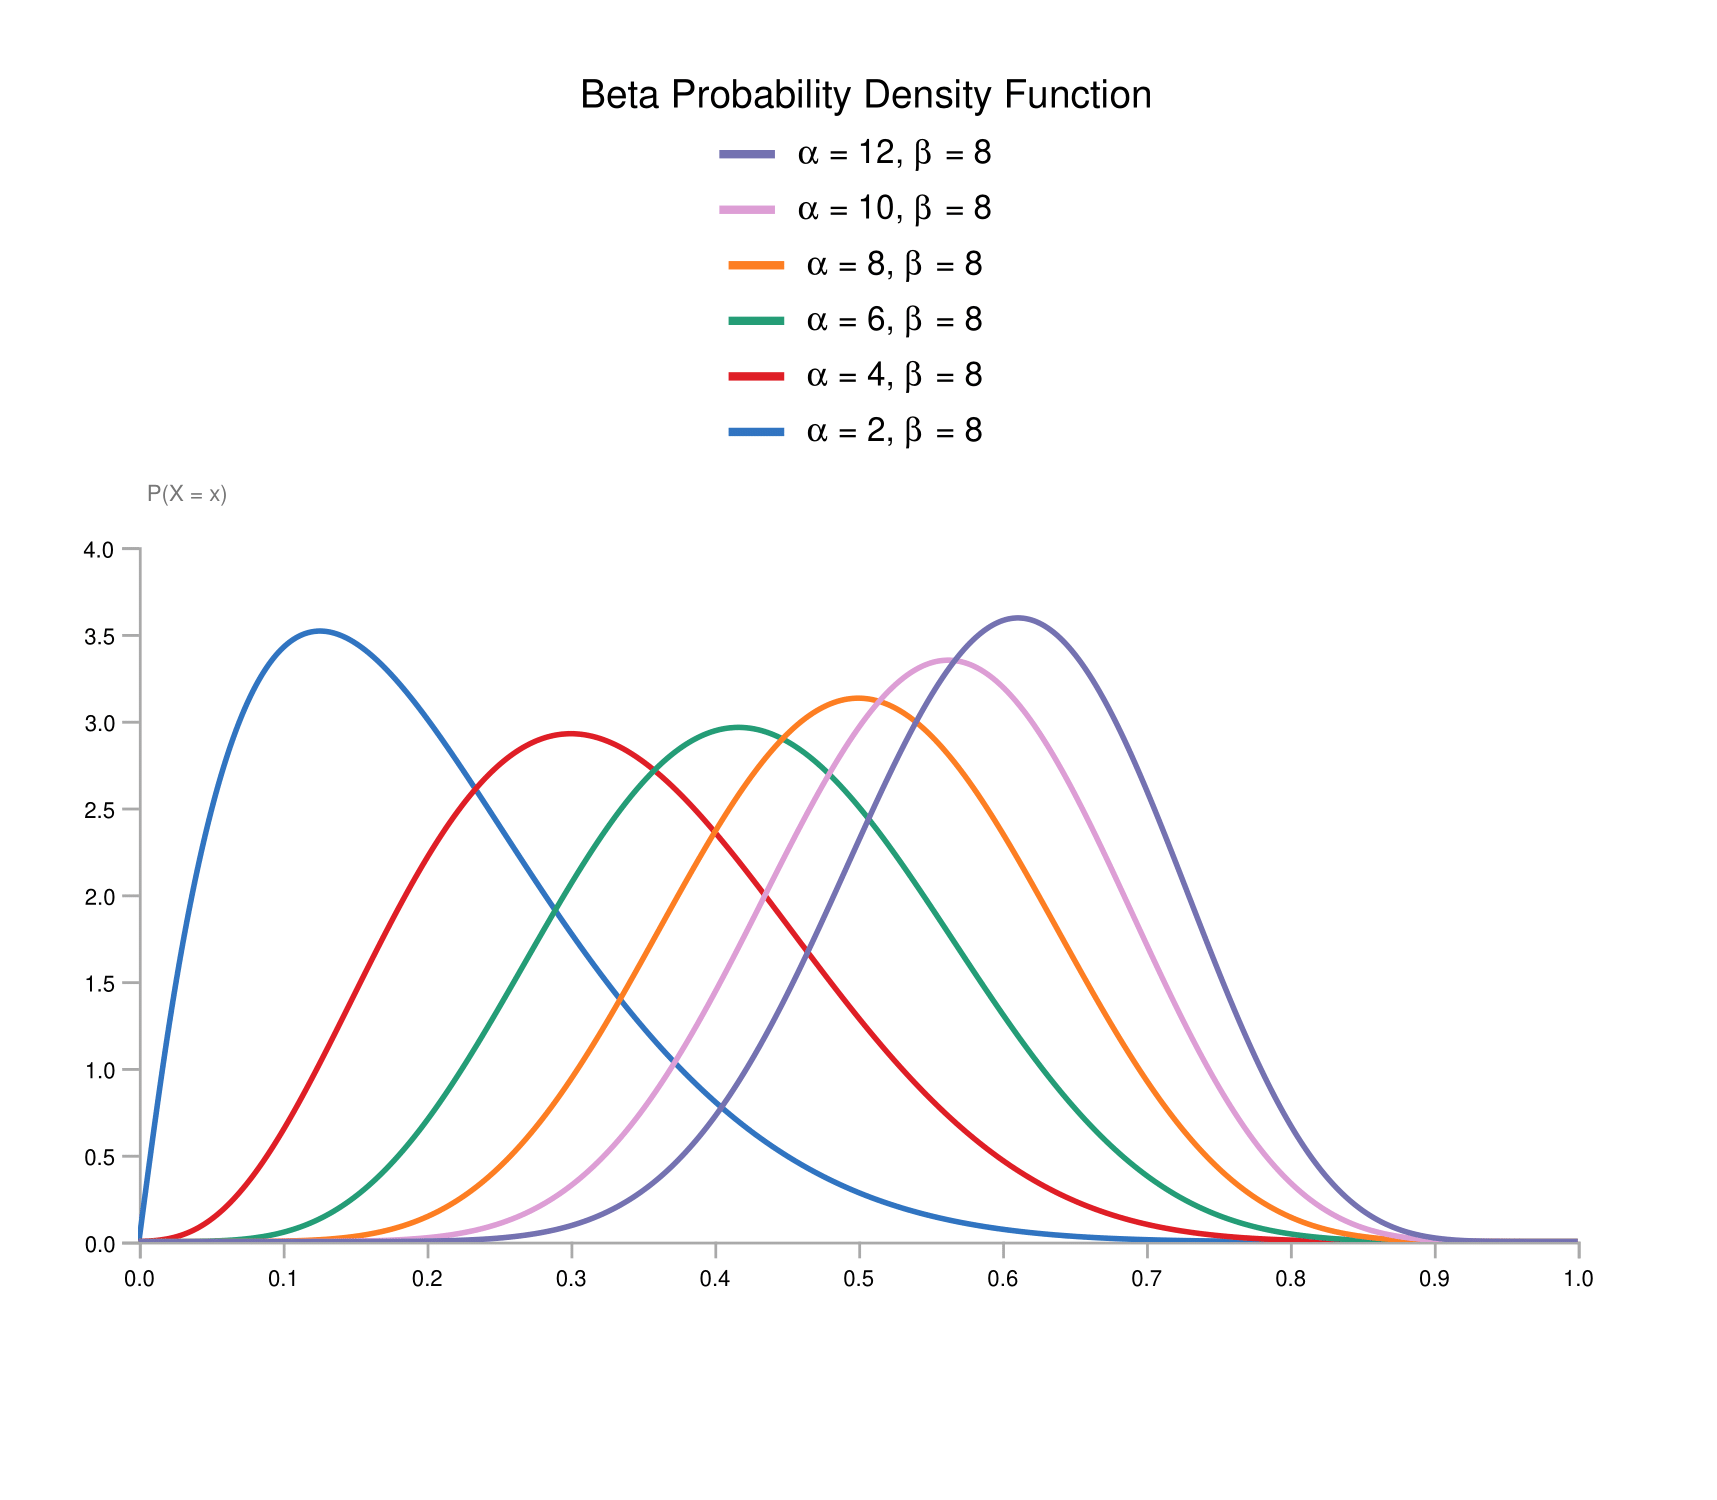
\includegraphics[width=6.26cm]{./images/chart (1)-1.png}\quad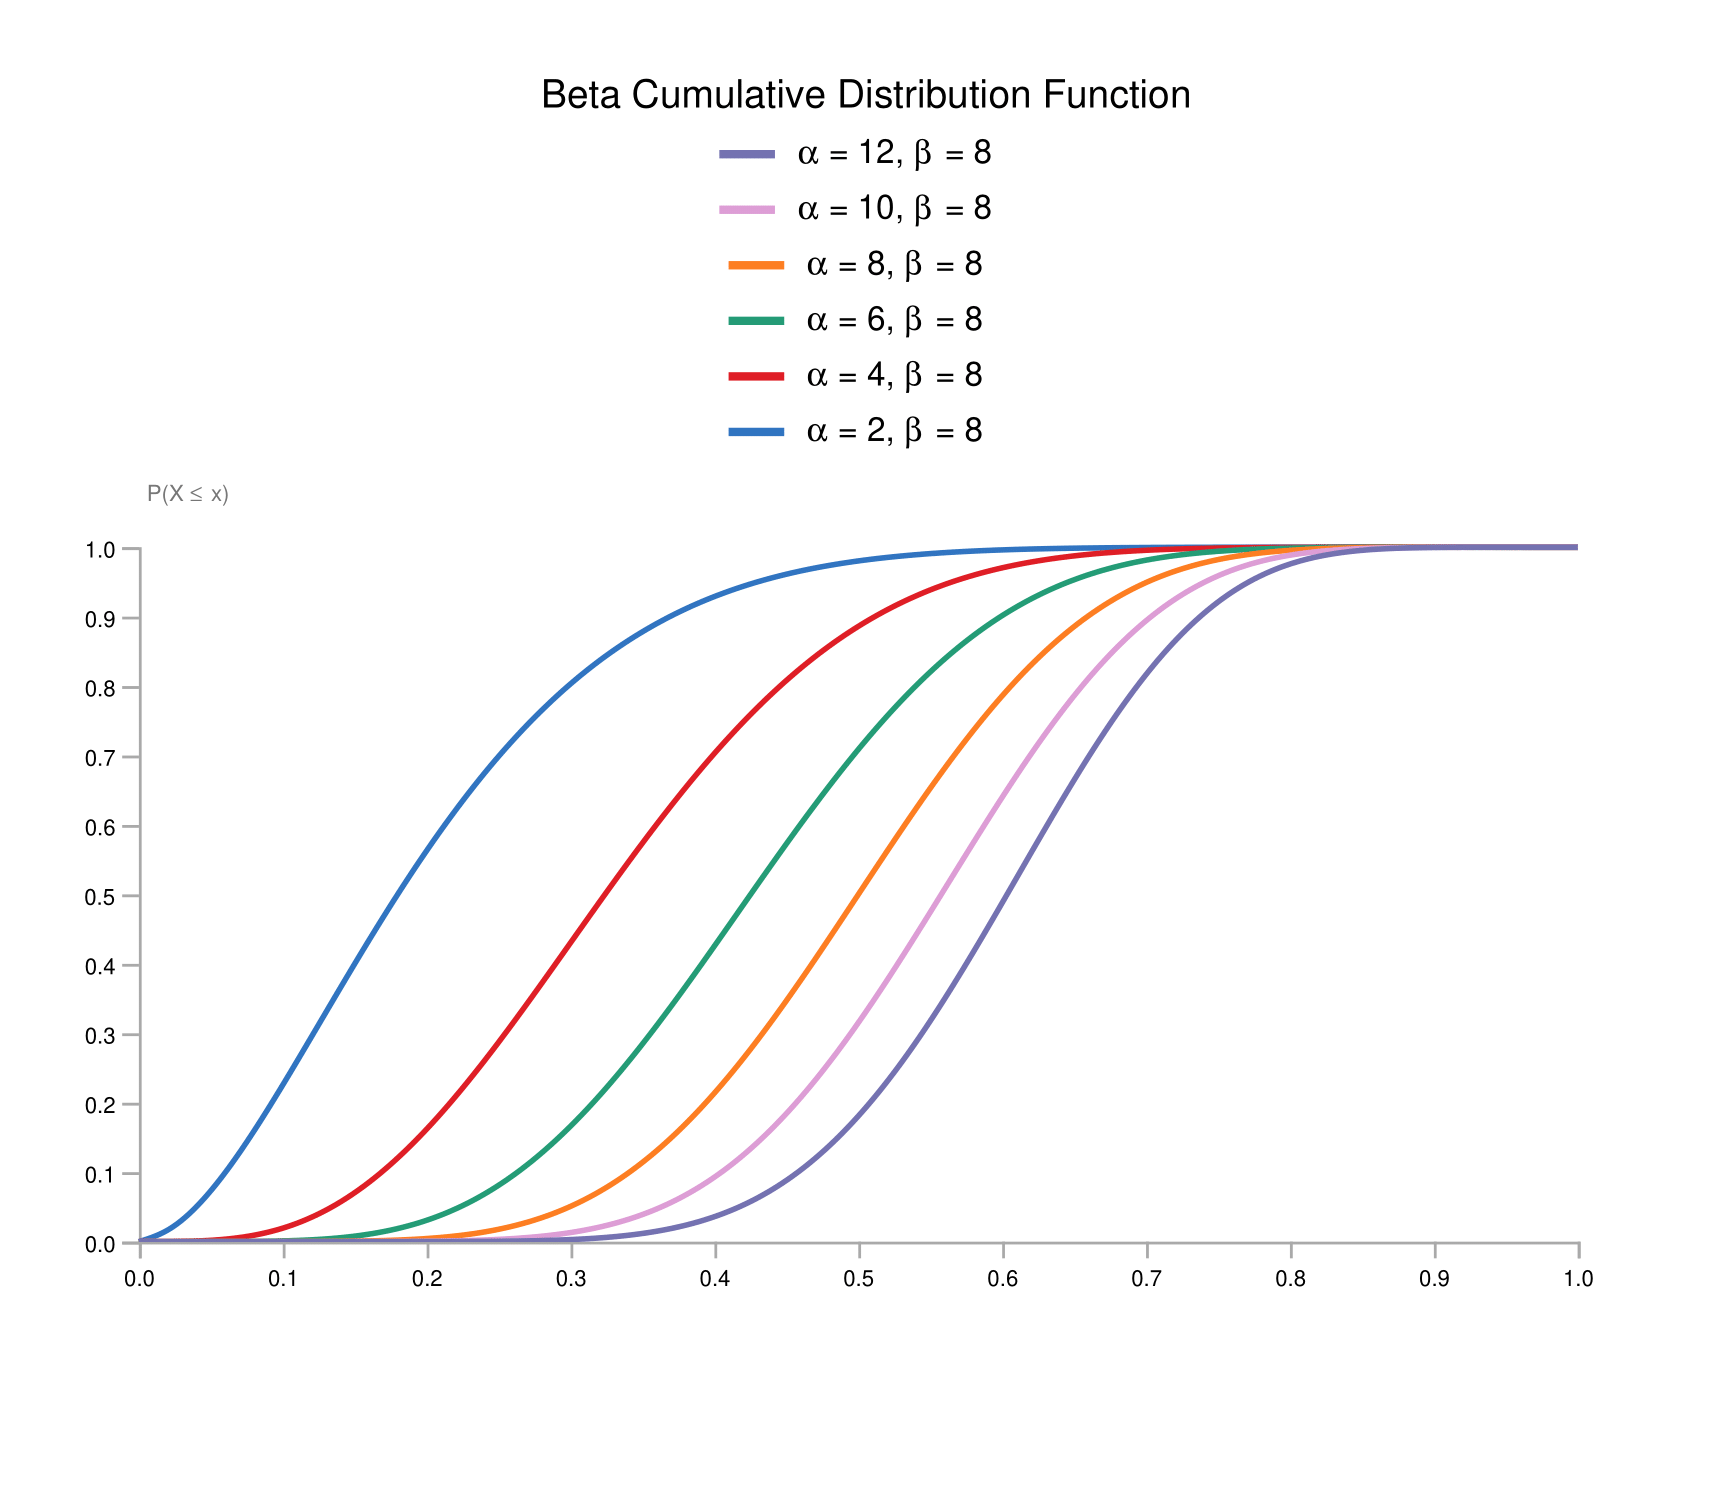
\includegraphics[width=6cm]{./images/chart (2)-1.png}
	\caption{Probability density function and cumulative distribution function of the Beta distributions considered in settings Synthetic B and Synthetic C.}
	\label{beta}
\end{figure}

\subsection{Synthetic C}

In this setting, we model the common situation where high feedback discourage long persistency, as previously discussed in Chapter \ref{CF}. At each time t, the true length $l_{j,t}$ is sampled from a Beta distribution depending on the pulled arm $a_j$. For each arm $a_j$, the feedback is $R_j$ is set such that to higher Beta mean corresponds lower feedback. We set $T_{max}=50,100,150,200$. For each $T_{max}$ adopted, the experiment is repeated for 50 independent runs. The full description of the arms is provided in Table \ref{tabSC} where with $\mu_{T_{max}}$ we indicate the expected pull reward in the configuration where $T_{max}$ is adopted.



\begin{table}[H]
	\centering
	\caption{Description of the arms in setting Synthetic C.}
	
	\begin{tabular}{|c|cccccc|}
		\hline
		\textbf{Arm}          & $a_0$ & $a_1$ & $a_2$ & $a_3$ & $a_4$ & $a_5$ \\ \hline
		\textbf{R}            & 6     & 5     & 4     & 3     & 2     & 1     \\
		$\boldsymbol{\alpha}$ & 2     & 4     & 6     & 8     & 10    & 12    \\
		$\boldsymbol{\beta}$  & 8     & 8     & 8     & 8     & 8     & 8     \\
		$\boldsymbol{\mu_{50}}$    & 10.50 & 17.17 & 21.93 & 25.50 & 28.28 & 30.3  \\ 
		$\boldsymbol{\mu_{100}}$    & 10.50 & 17.17 & 21.93 & 25.50 & 28.28 & 30.3  \\ 
		$\boldsymbol{\mu_{150}}$    & 10.50 & 17.17 & 21.93 & 25.50 & 28.28 & 30.3  \\ 
		$\boldsymbol{\mu_{200}}$    & 10.50 & 17.17 & 21.93 & 25.50 & 28.28 & 30.3  \\ \hline
	\end{tabular}
	
	\label{tabSC}
\end{table}

\section{Results}

\begin{figure}[h]
	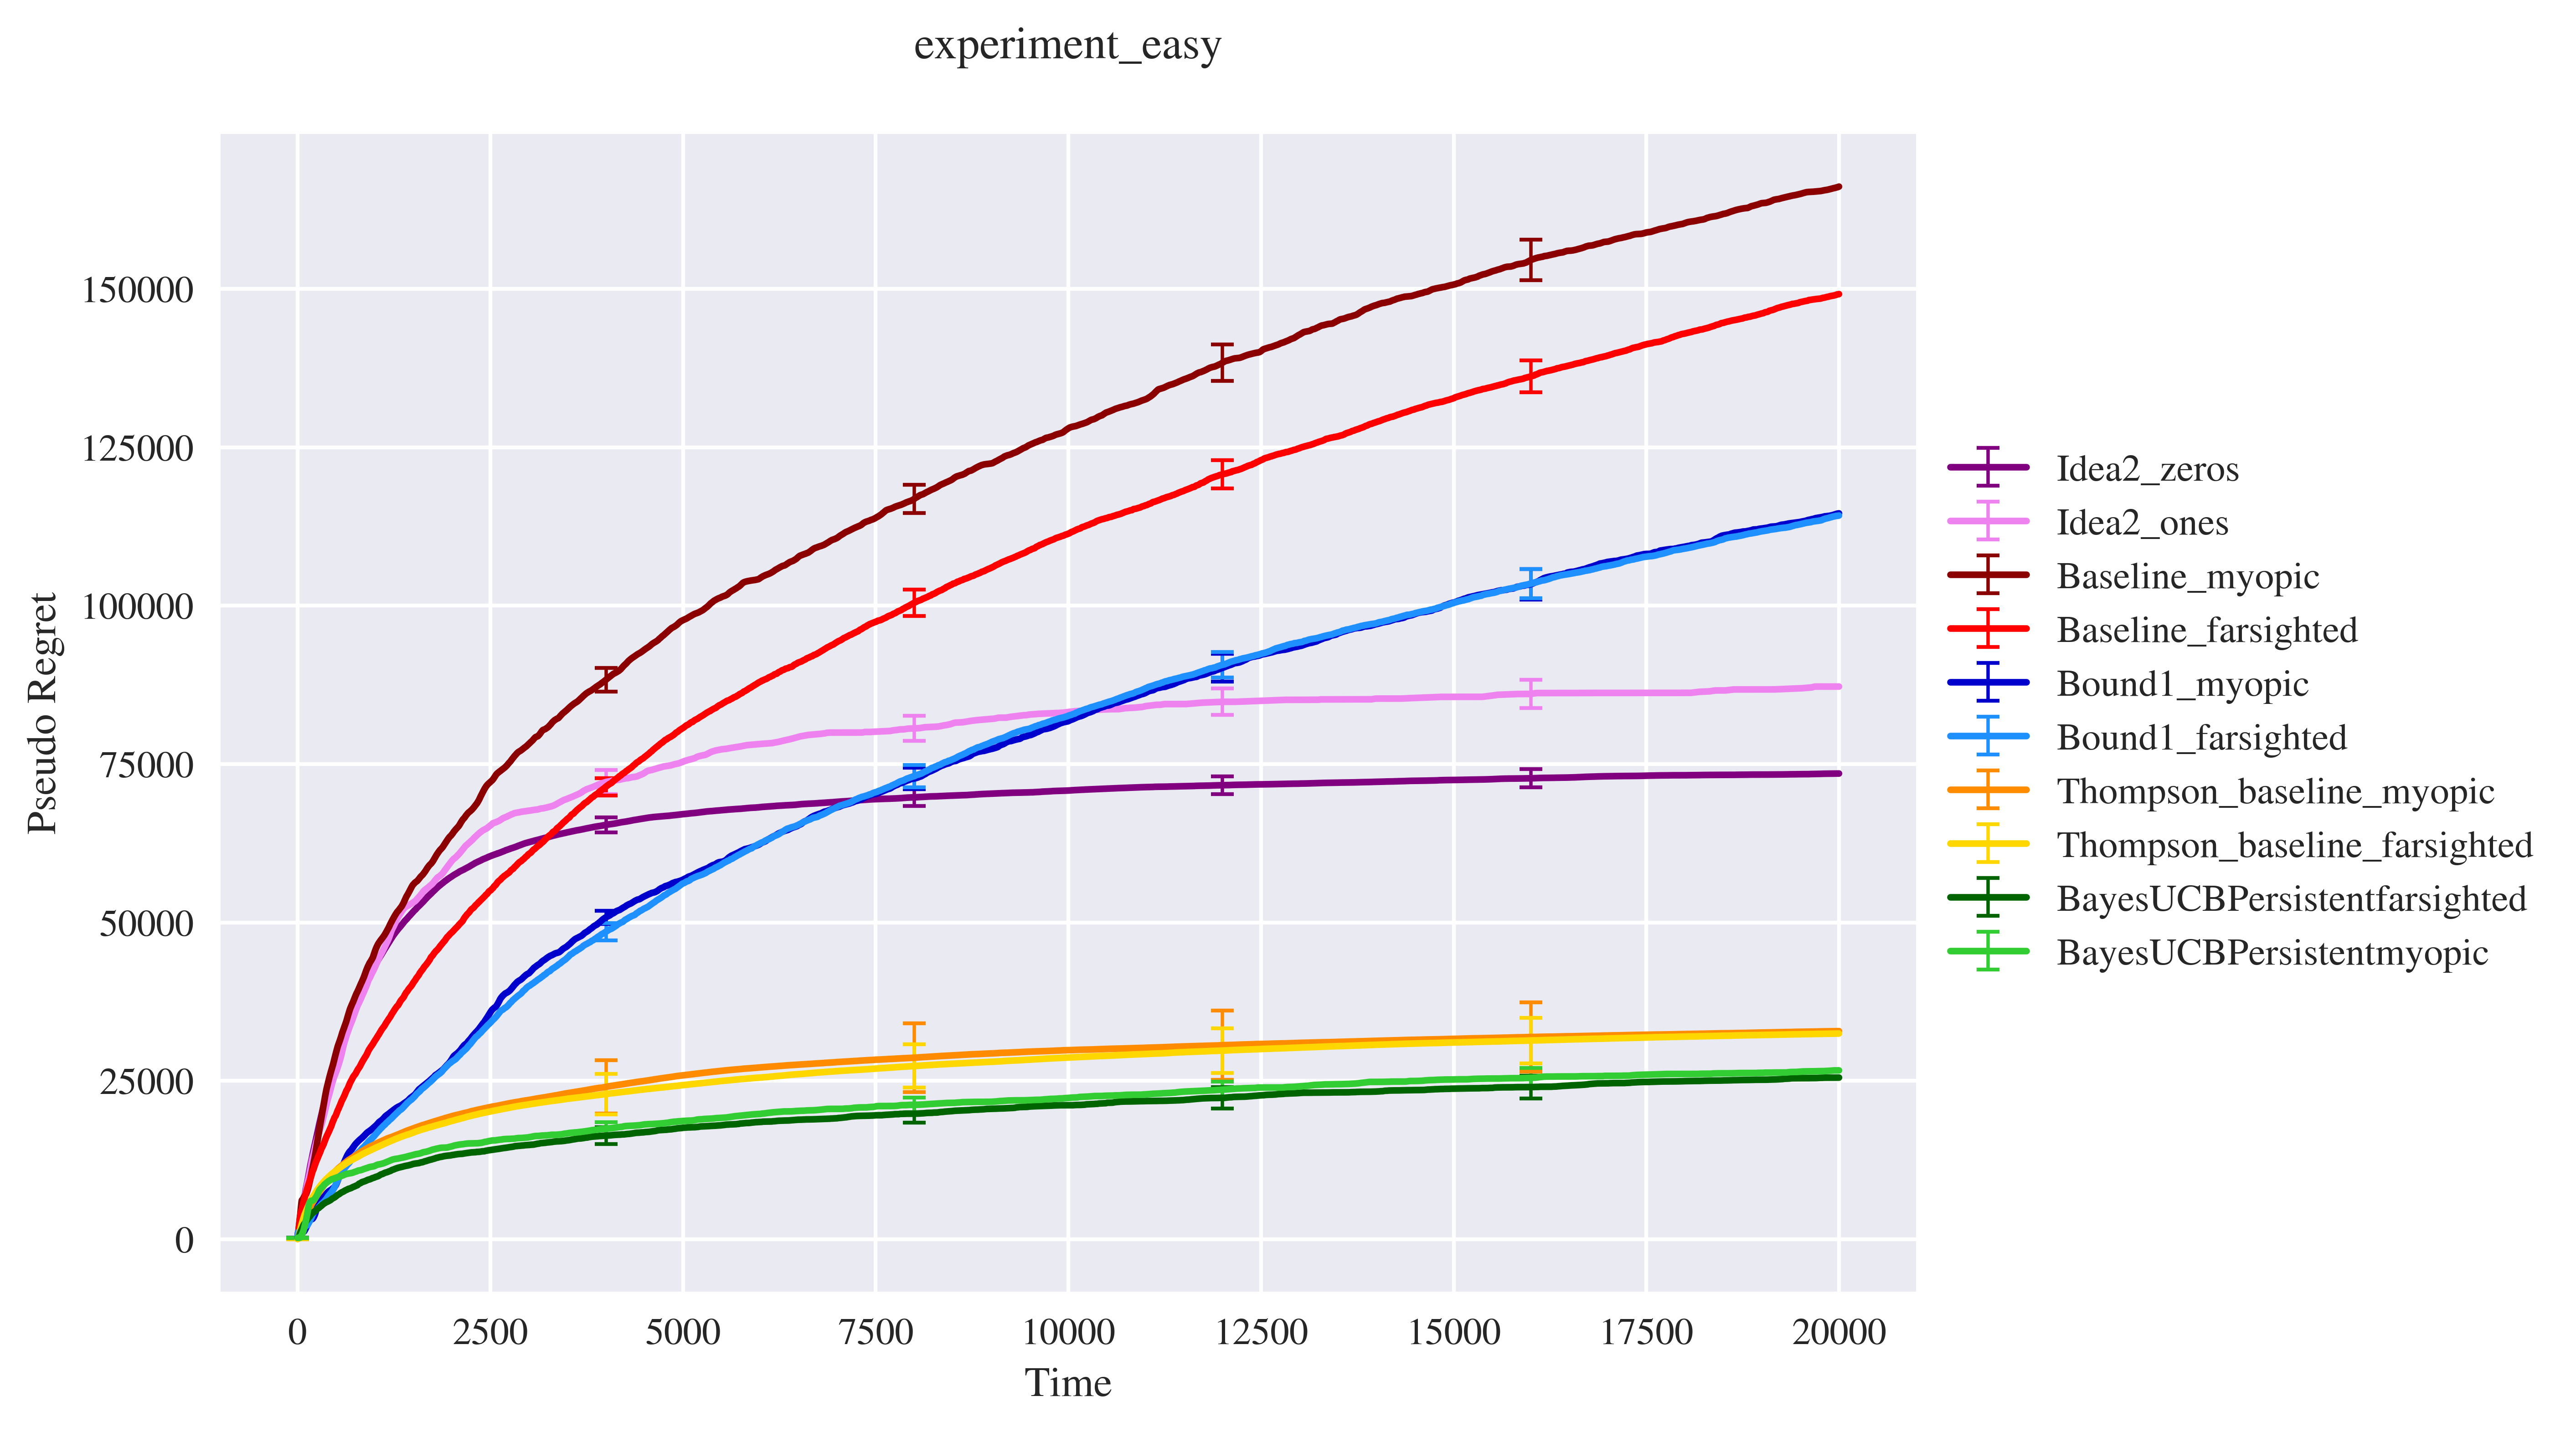
\includegraphics[width=16cm]{./images/experiment_easy ANALYTICS.png}
	\centering	
	\caption{SYNTHETIC A pseudo regret: beta uniformi (R: 1...10) 50 runs Tmax=50}
\end{figure}
\begin{figure}[h]
	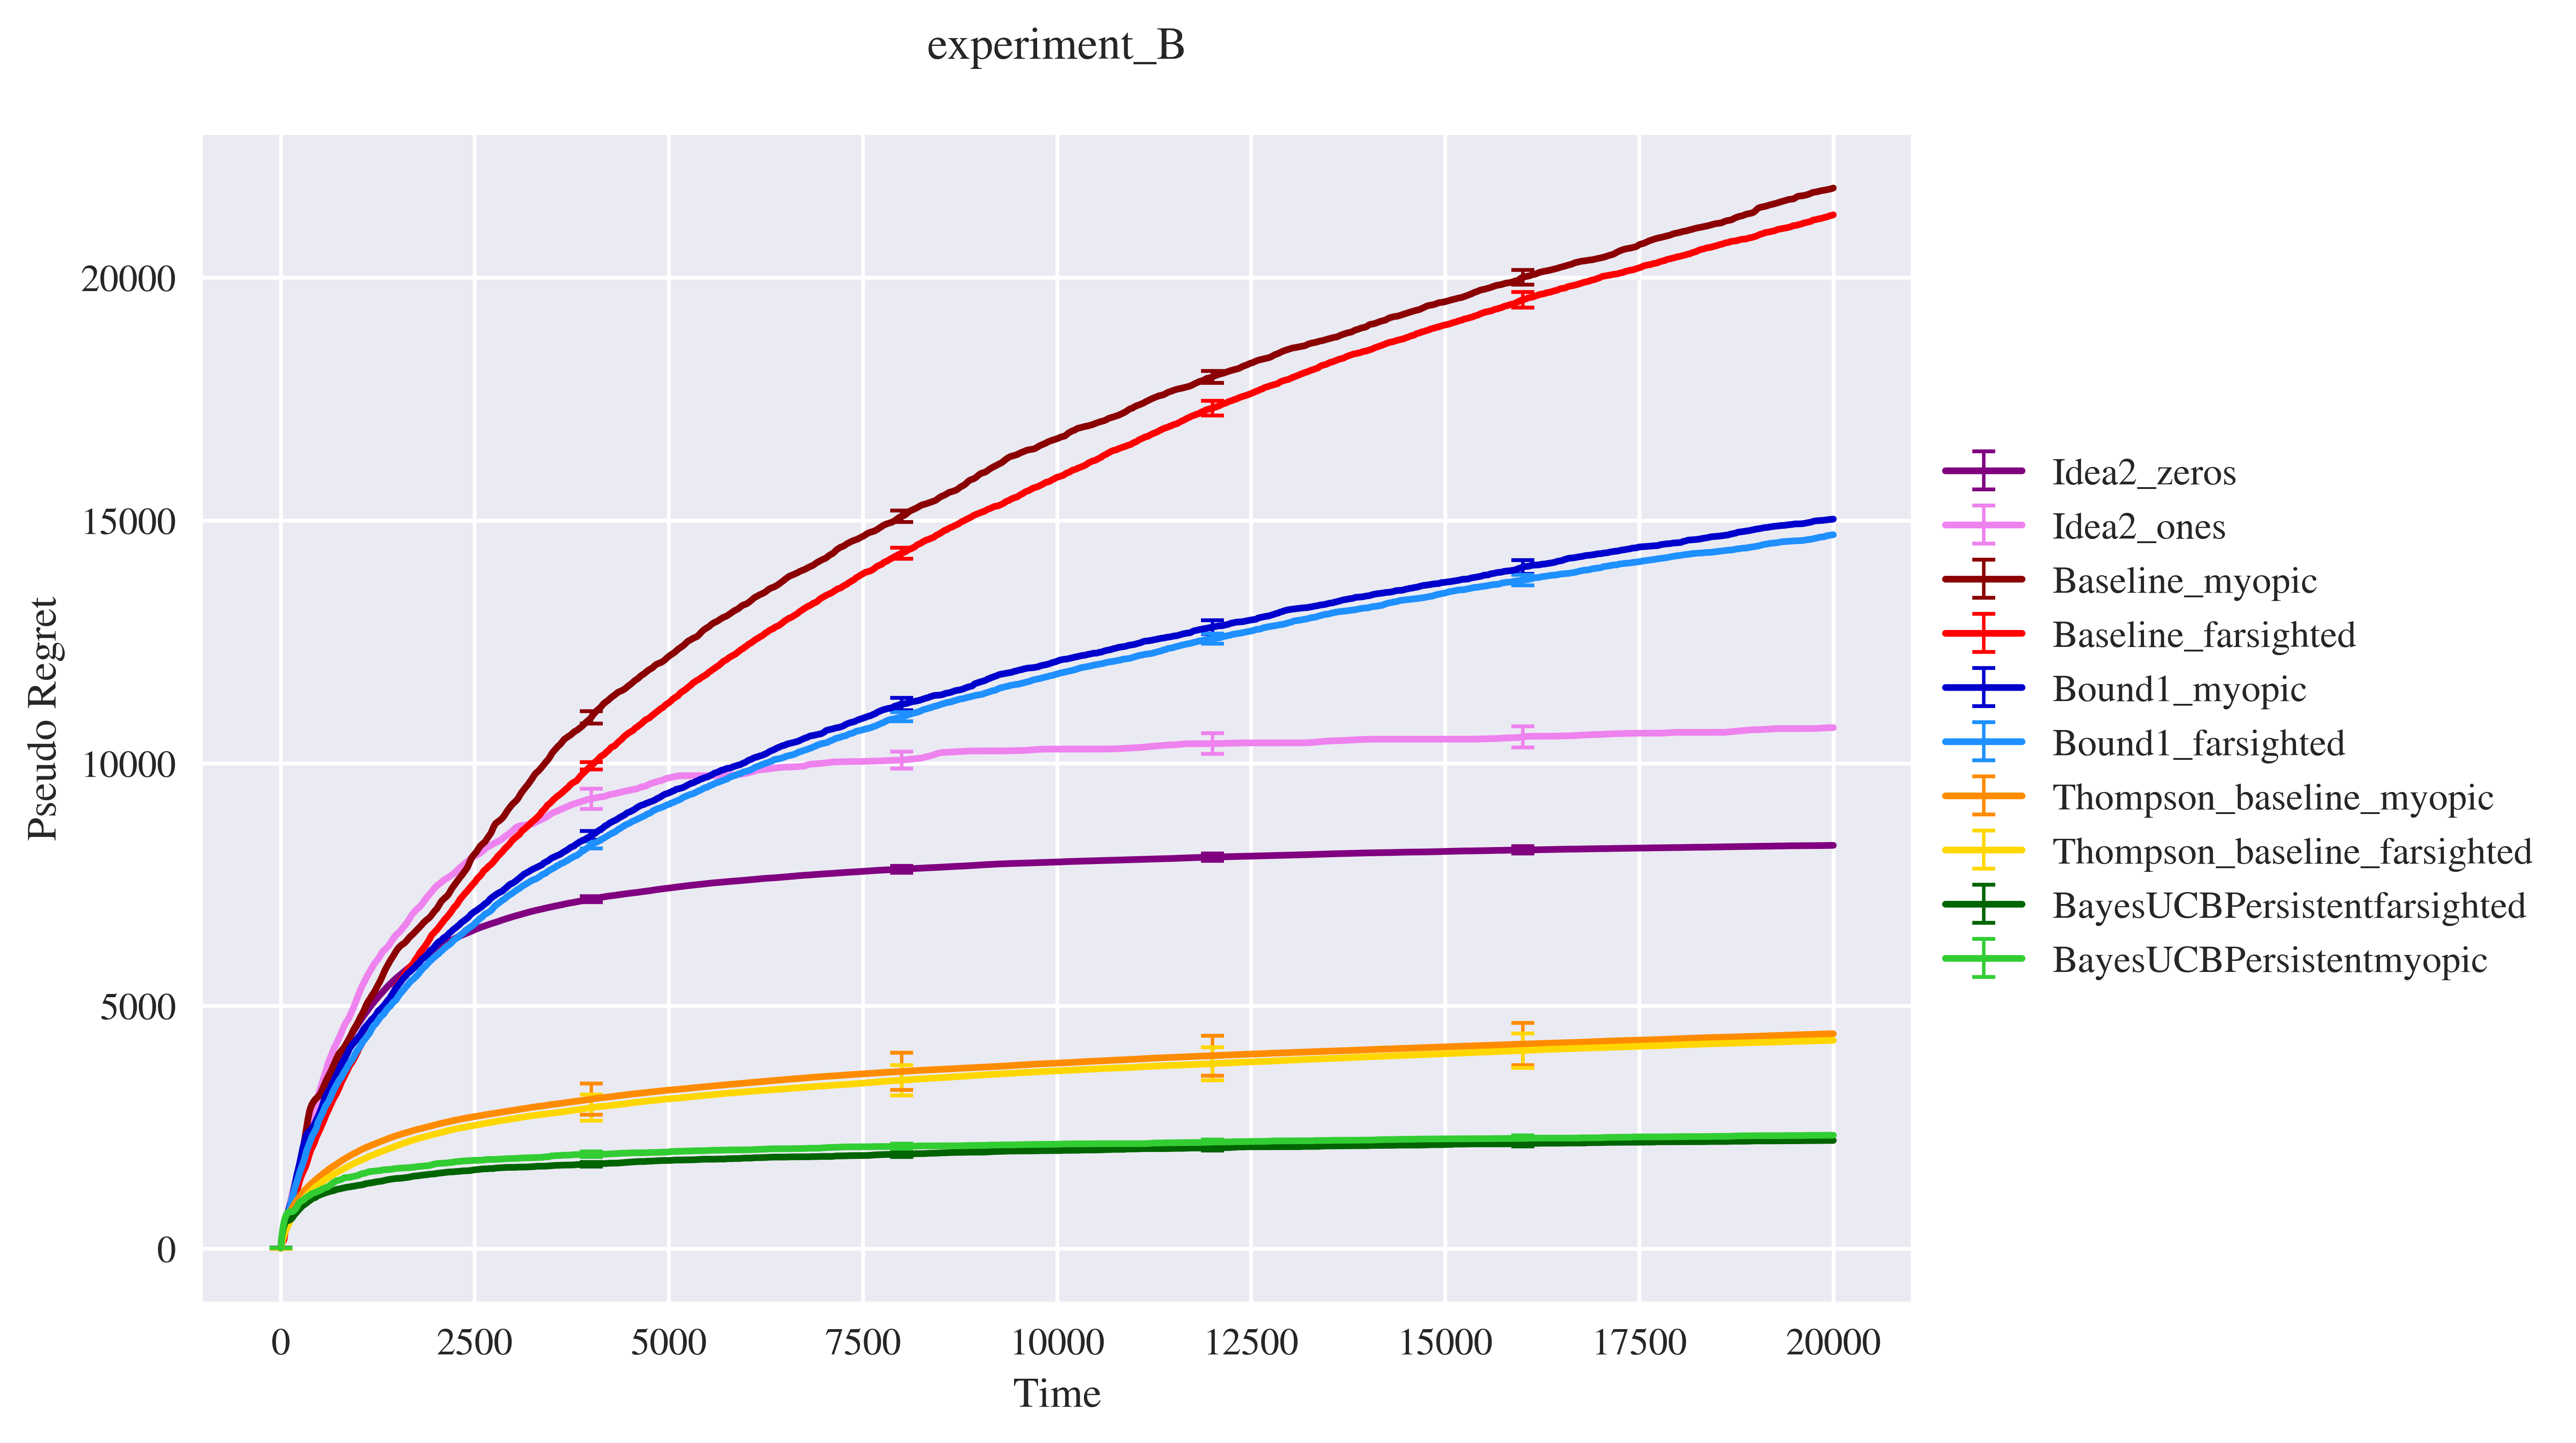
\includegraphics[width=16cm]{./images/experiment_B ANALYTICS.png}
	\centering	
	\caption{SYNTHETIC B pseudo regret: 50runs,  R fixed, Tmax=50, Beta "crescenti" }
\end{figure}

\begin{figure}
	\centering
	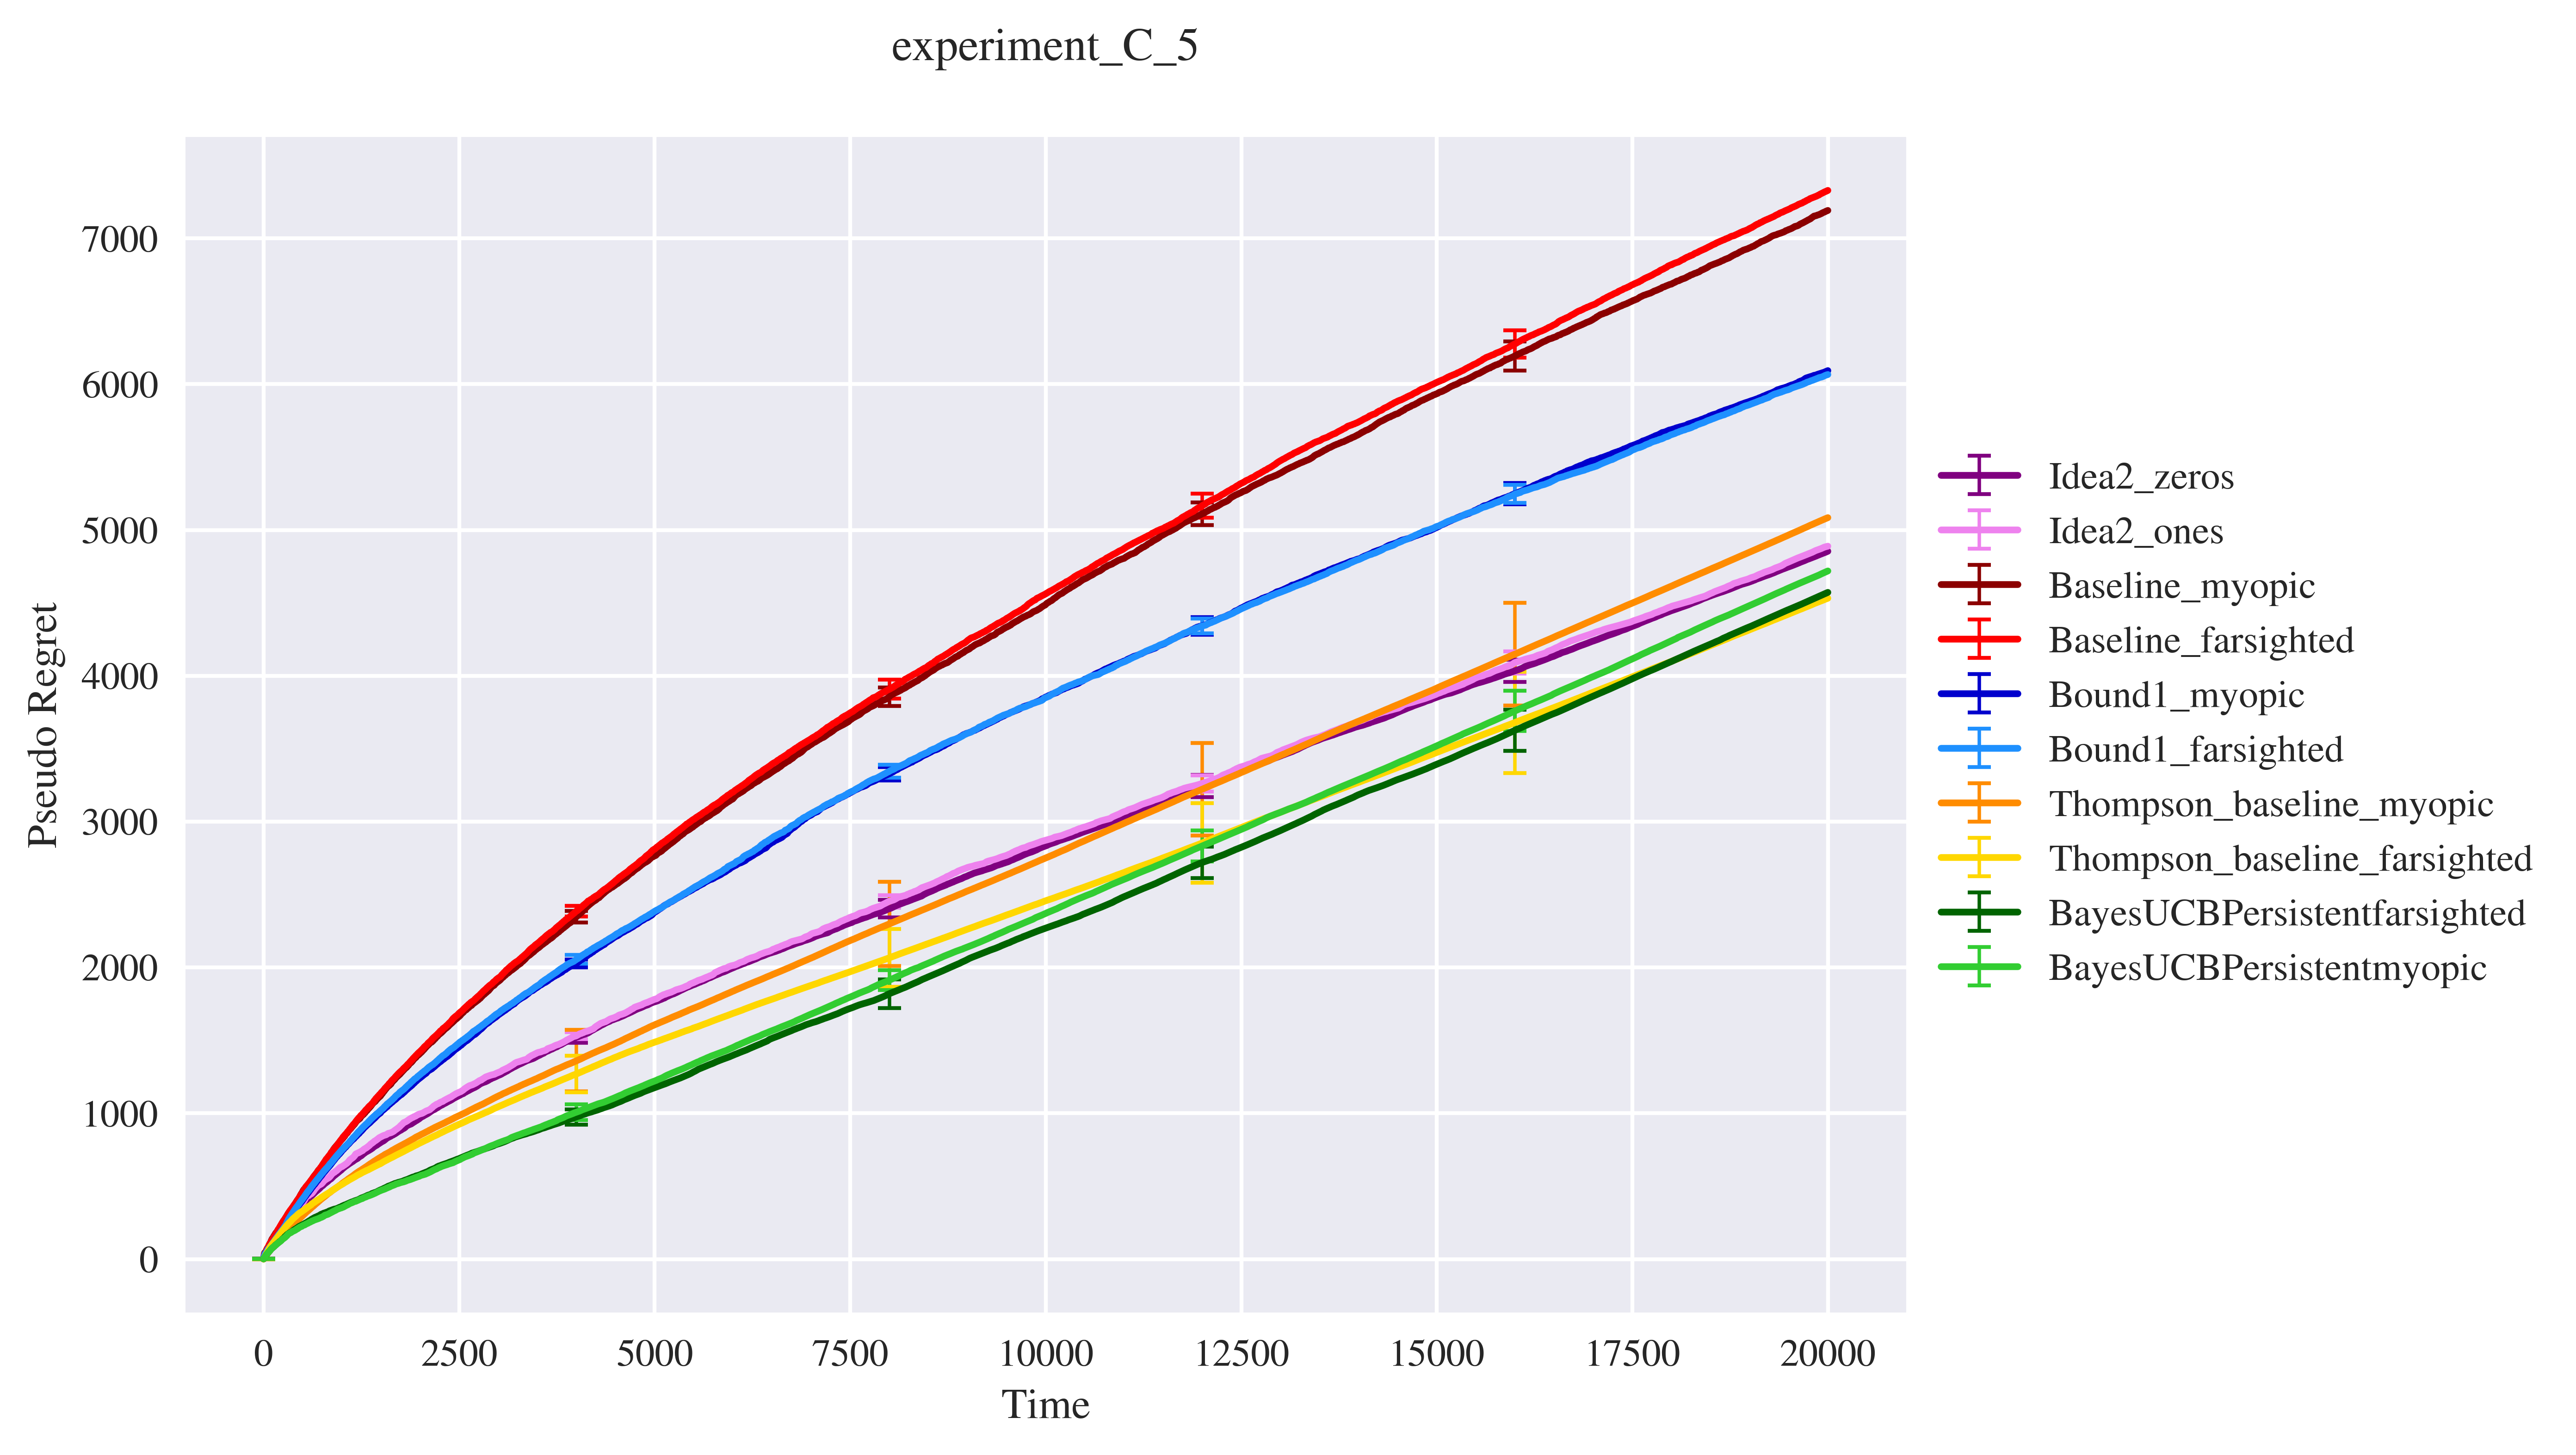
\includegraphics[width=6cm]{./images/C/experiment_C_5 ANALYTICS.png}\quad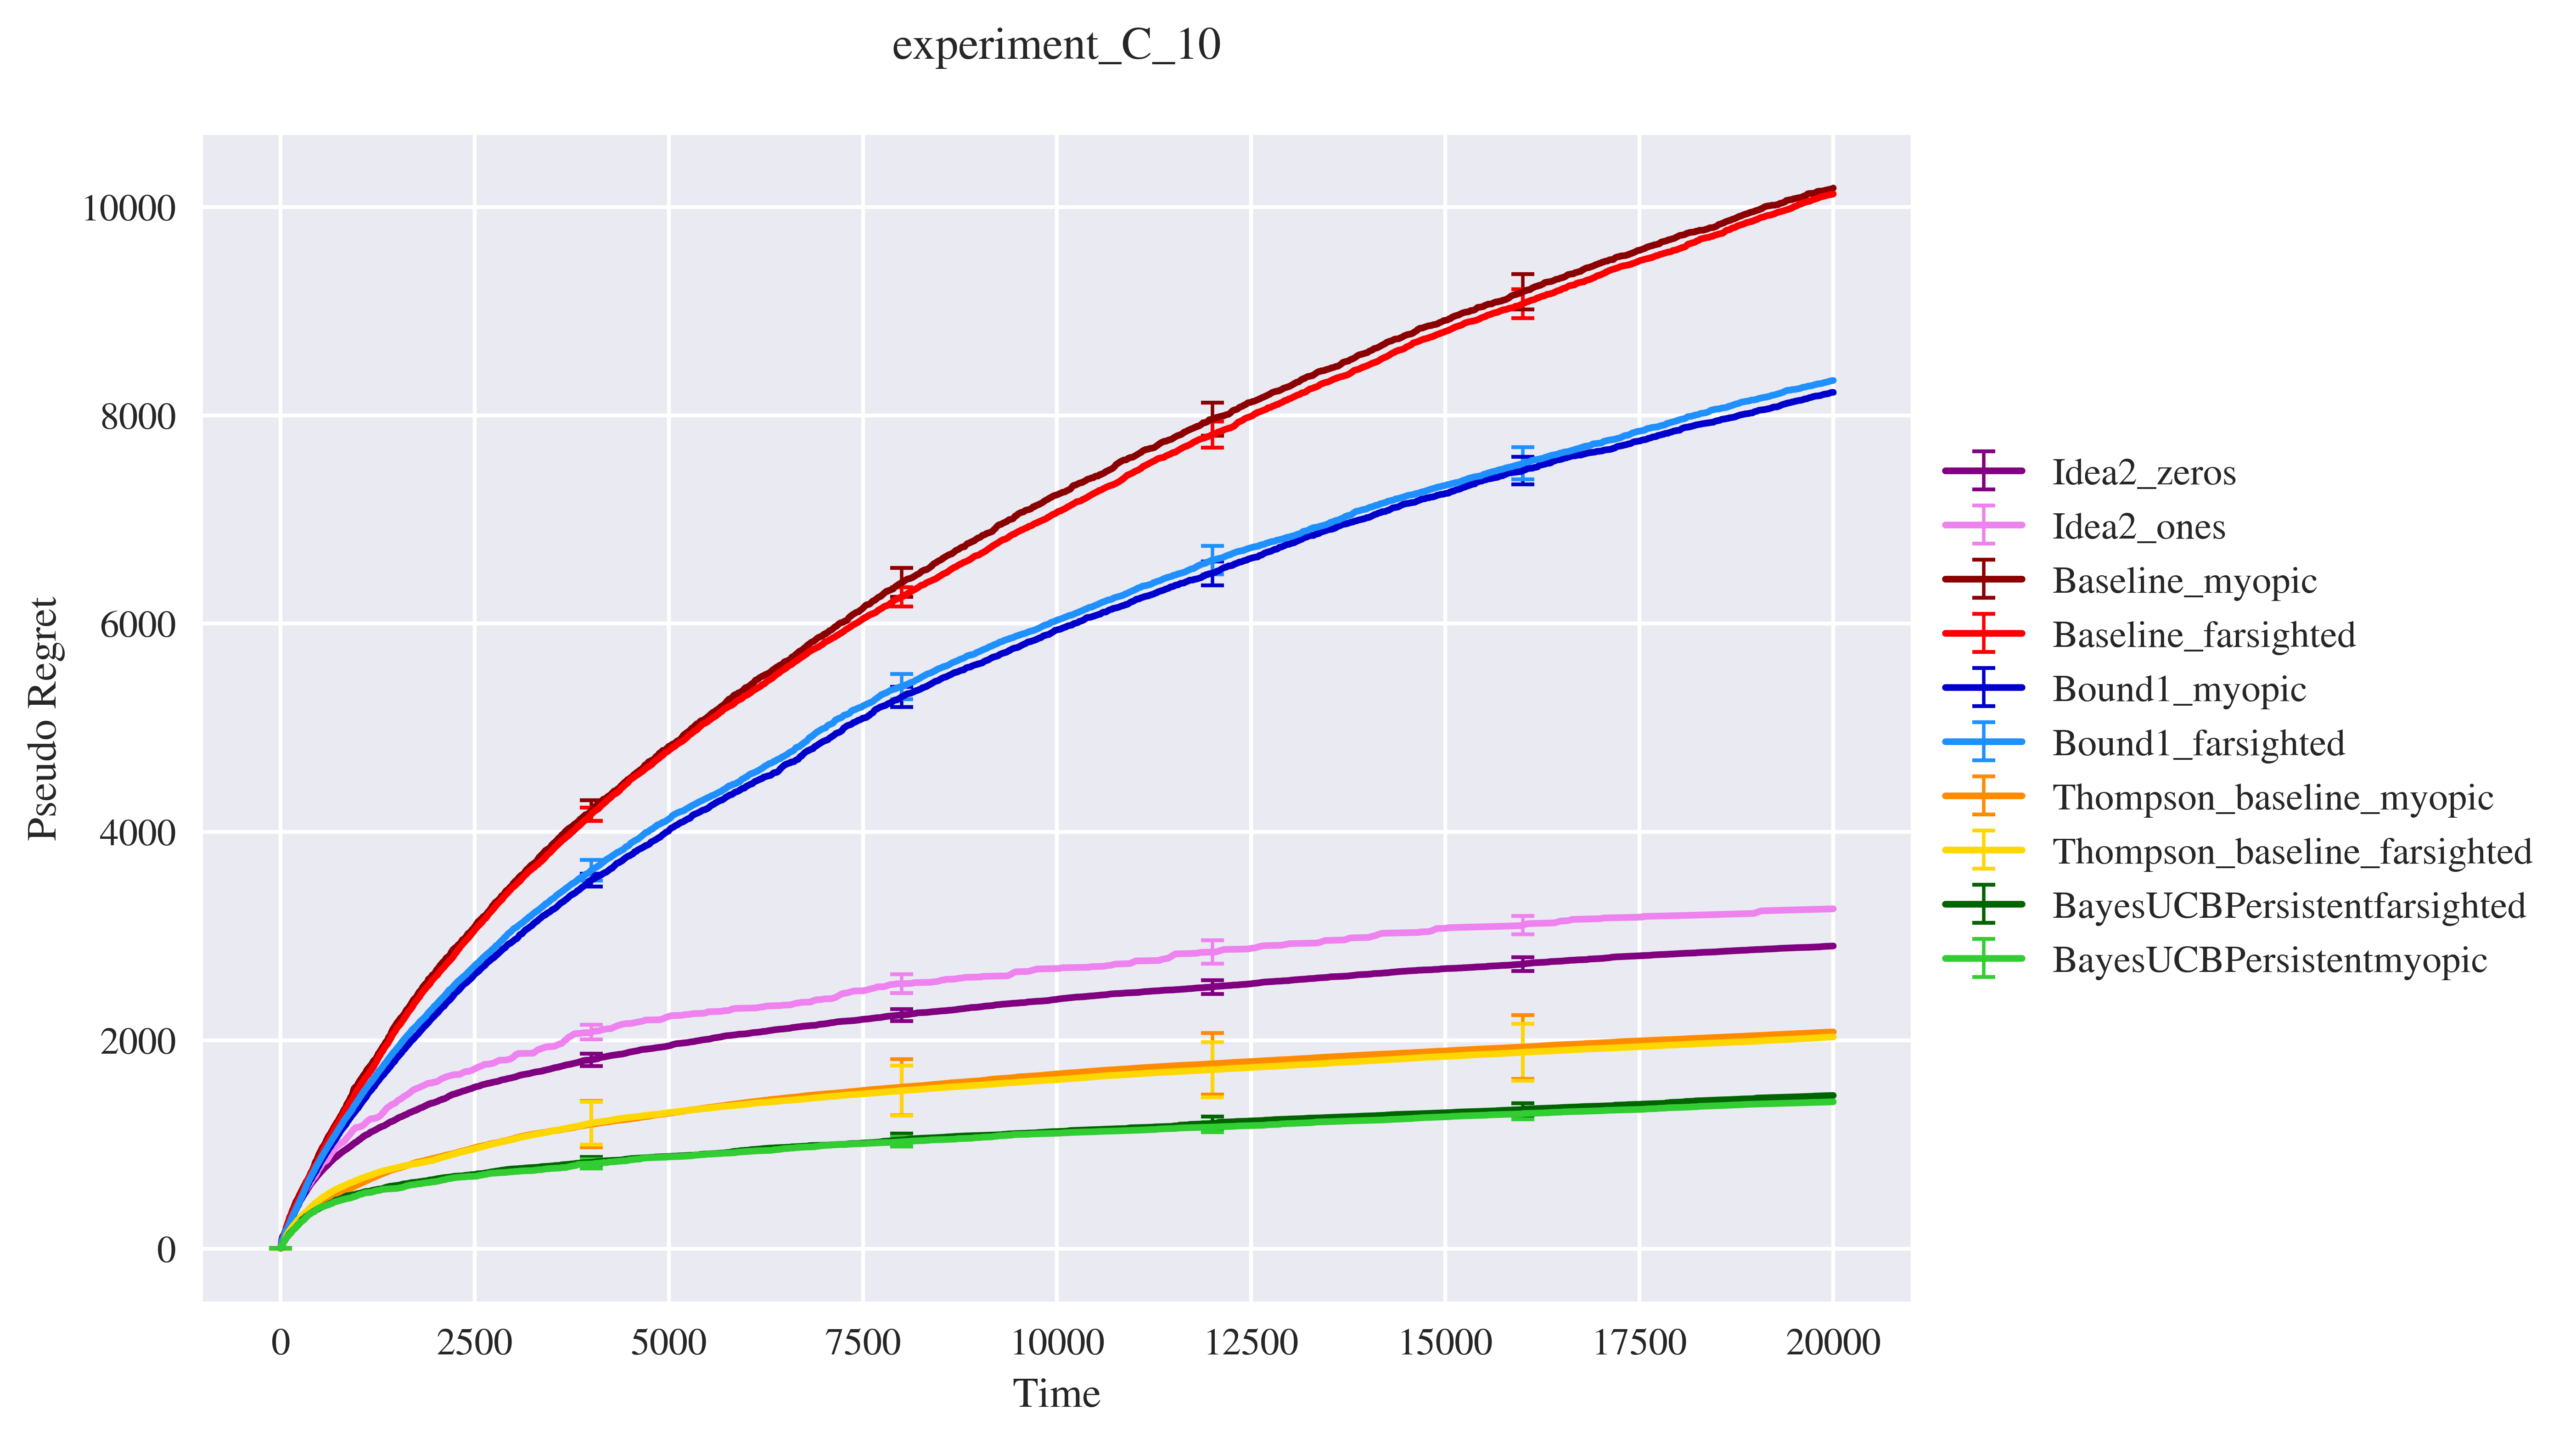
\includegraphics[width=6cm]{./images/C/experiment_C_10 ANALYTICS.png} 
	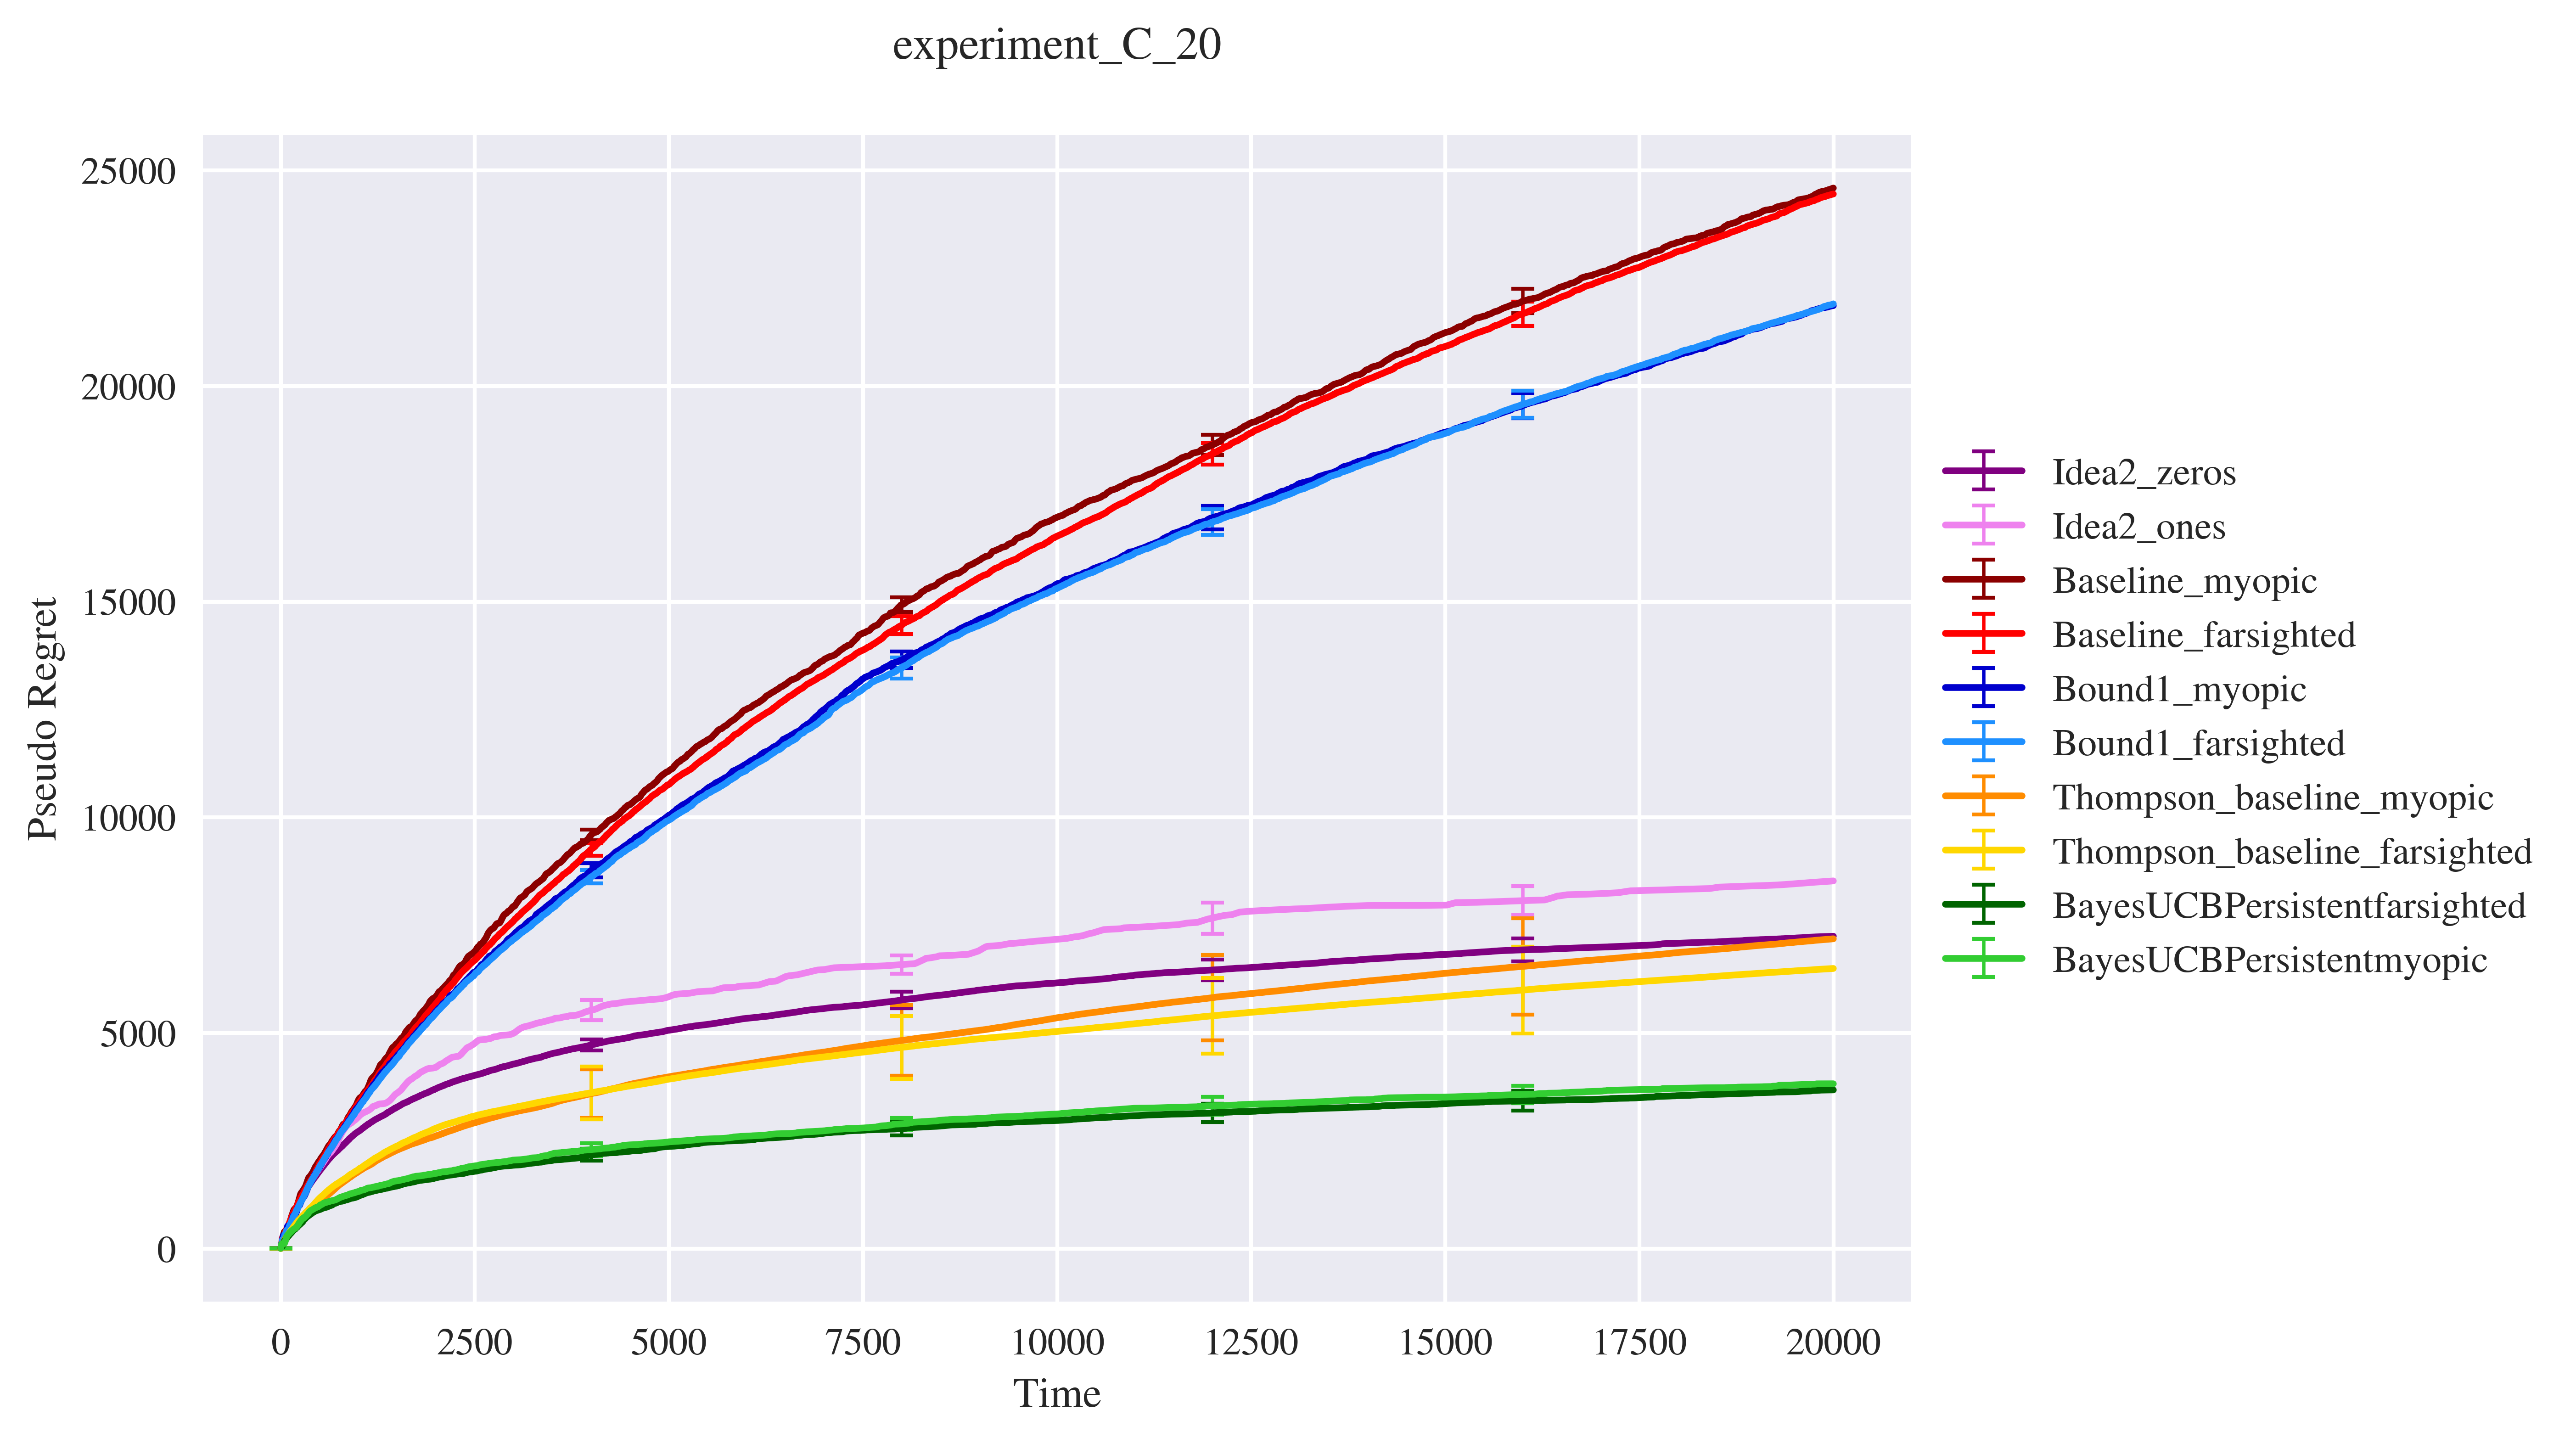
\includegraphics[width=6cm]{./images/C/experiment_C_20 ANALYTICS.png}\quad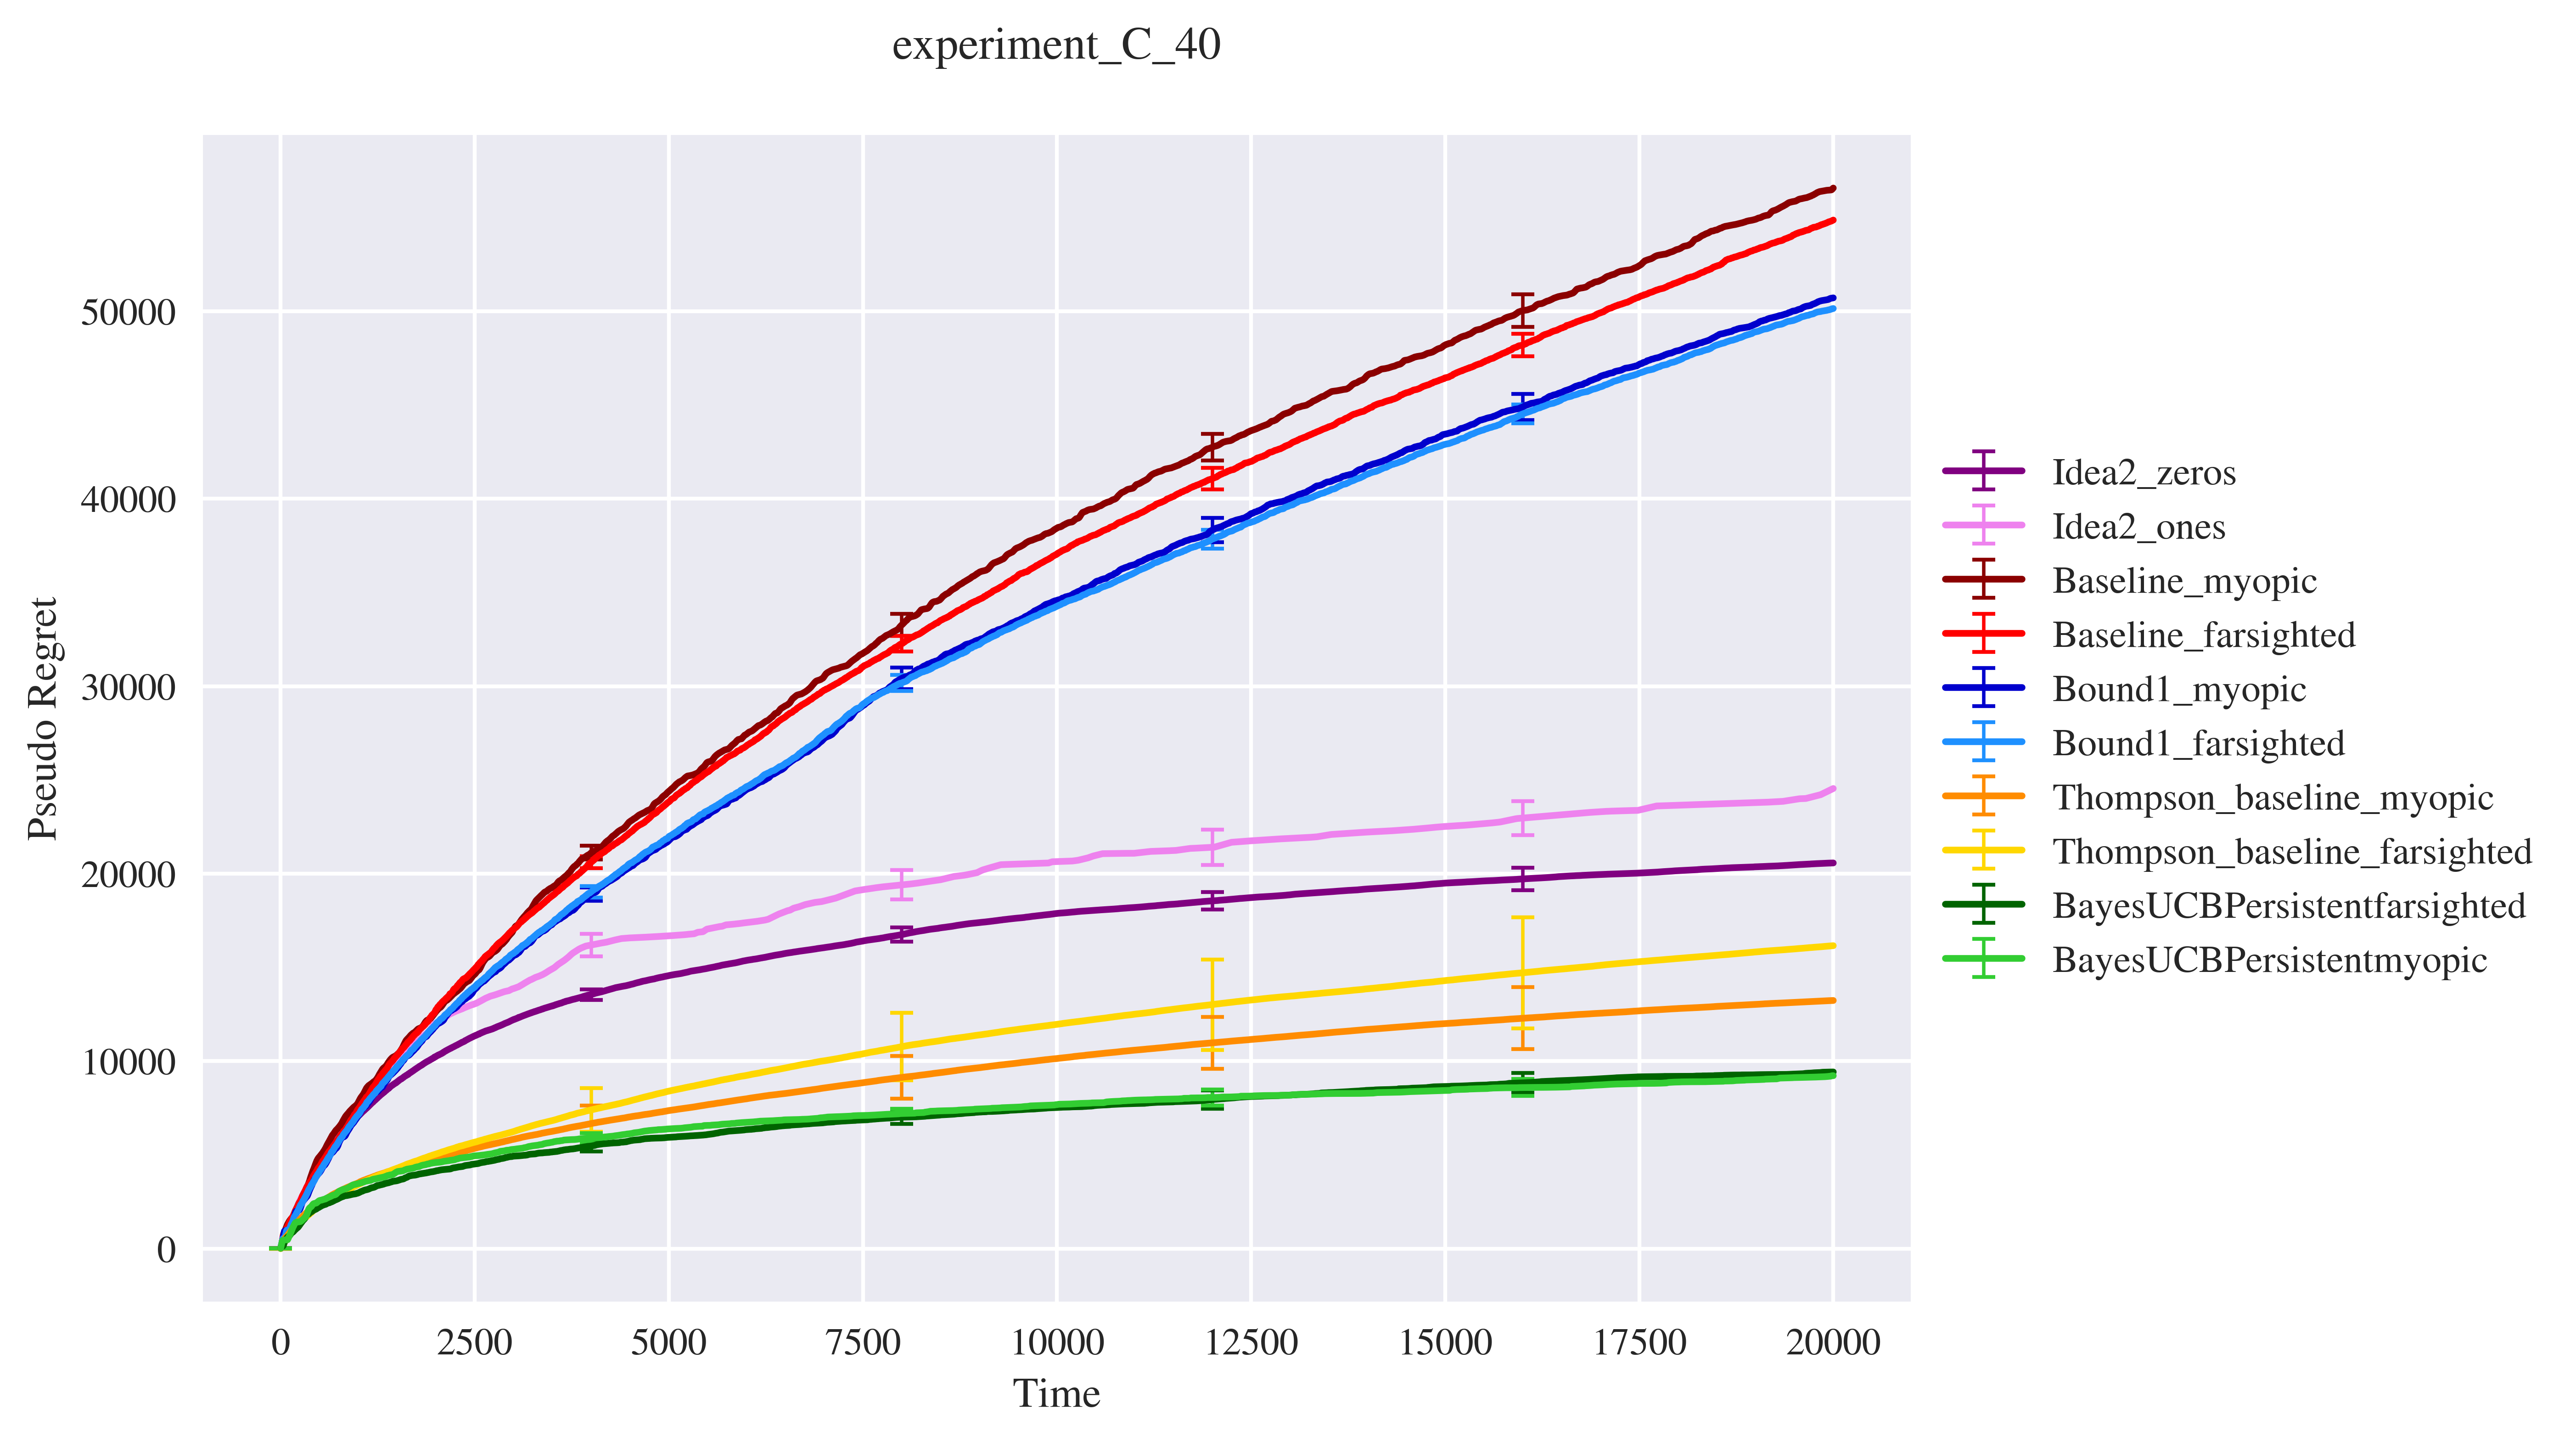
\includegraphics[width=6cm]{./images/C/experiment_C_40 ANALYTICS.png}
	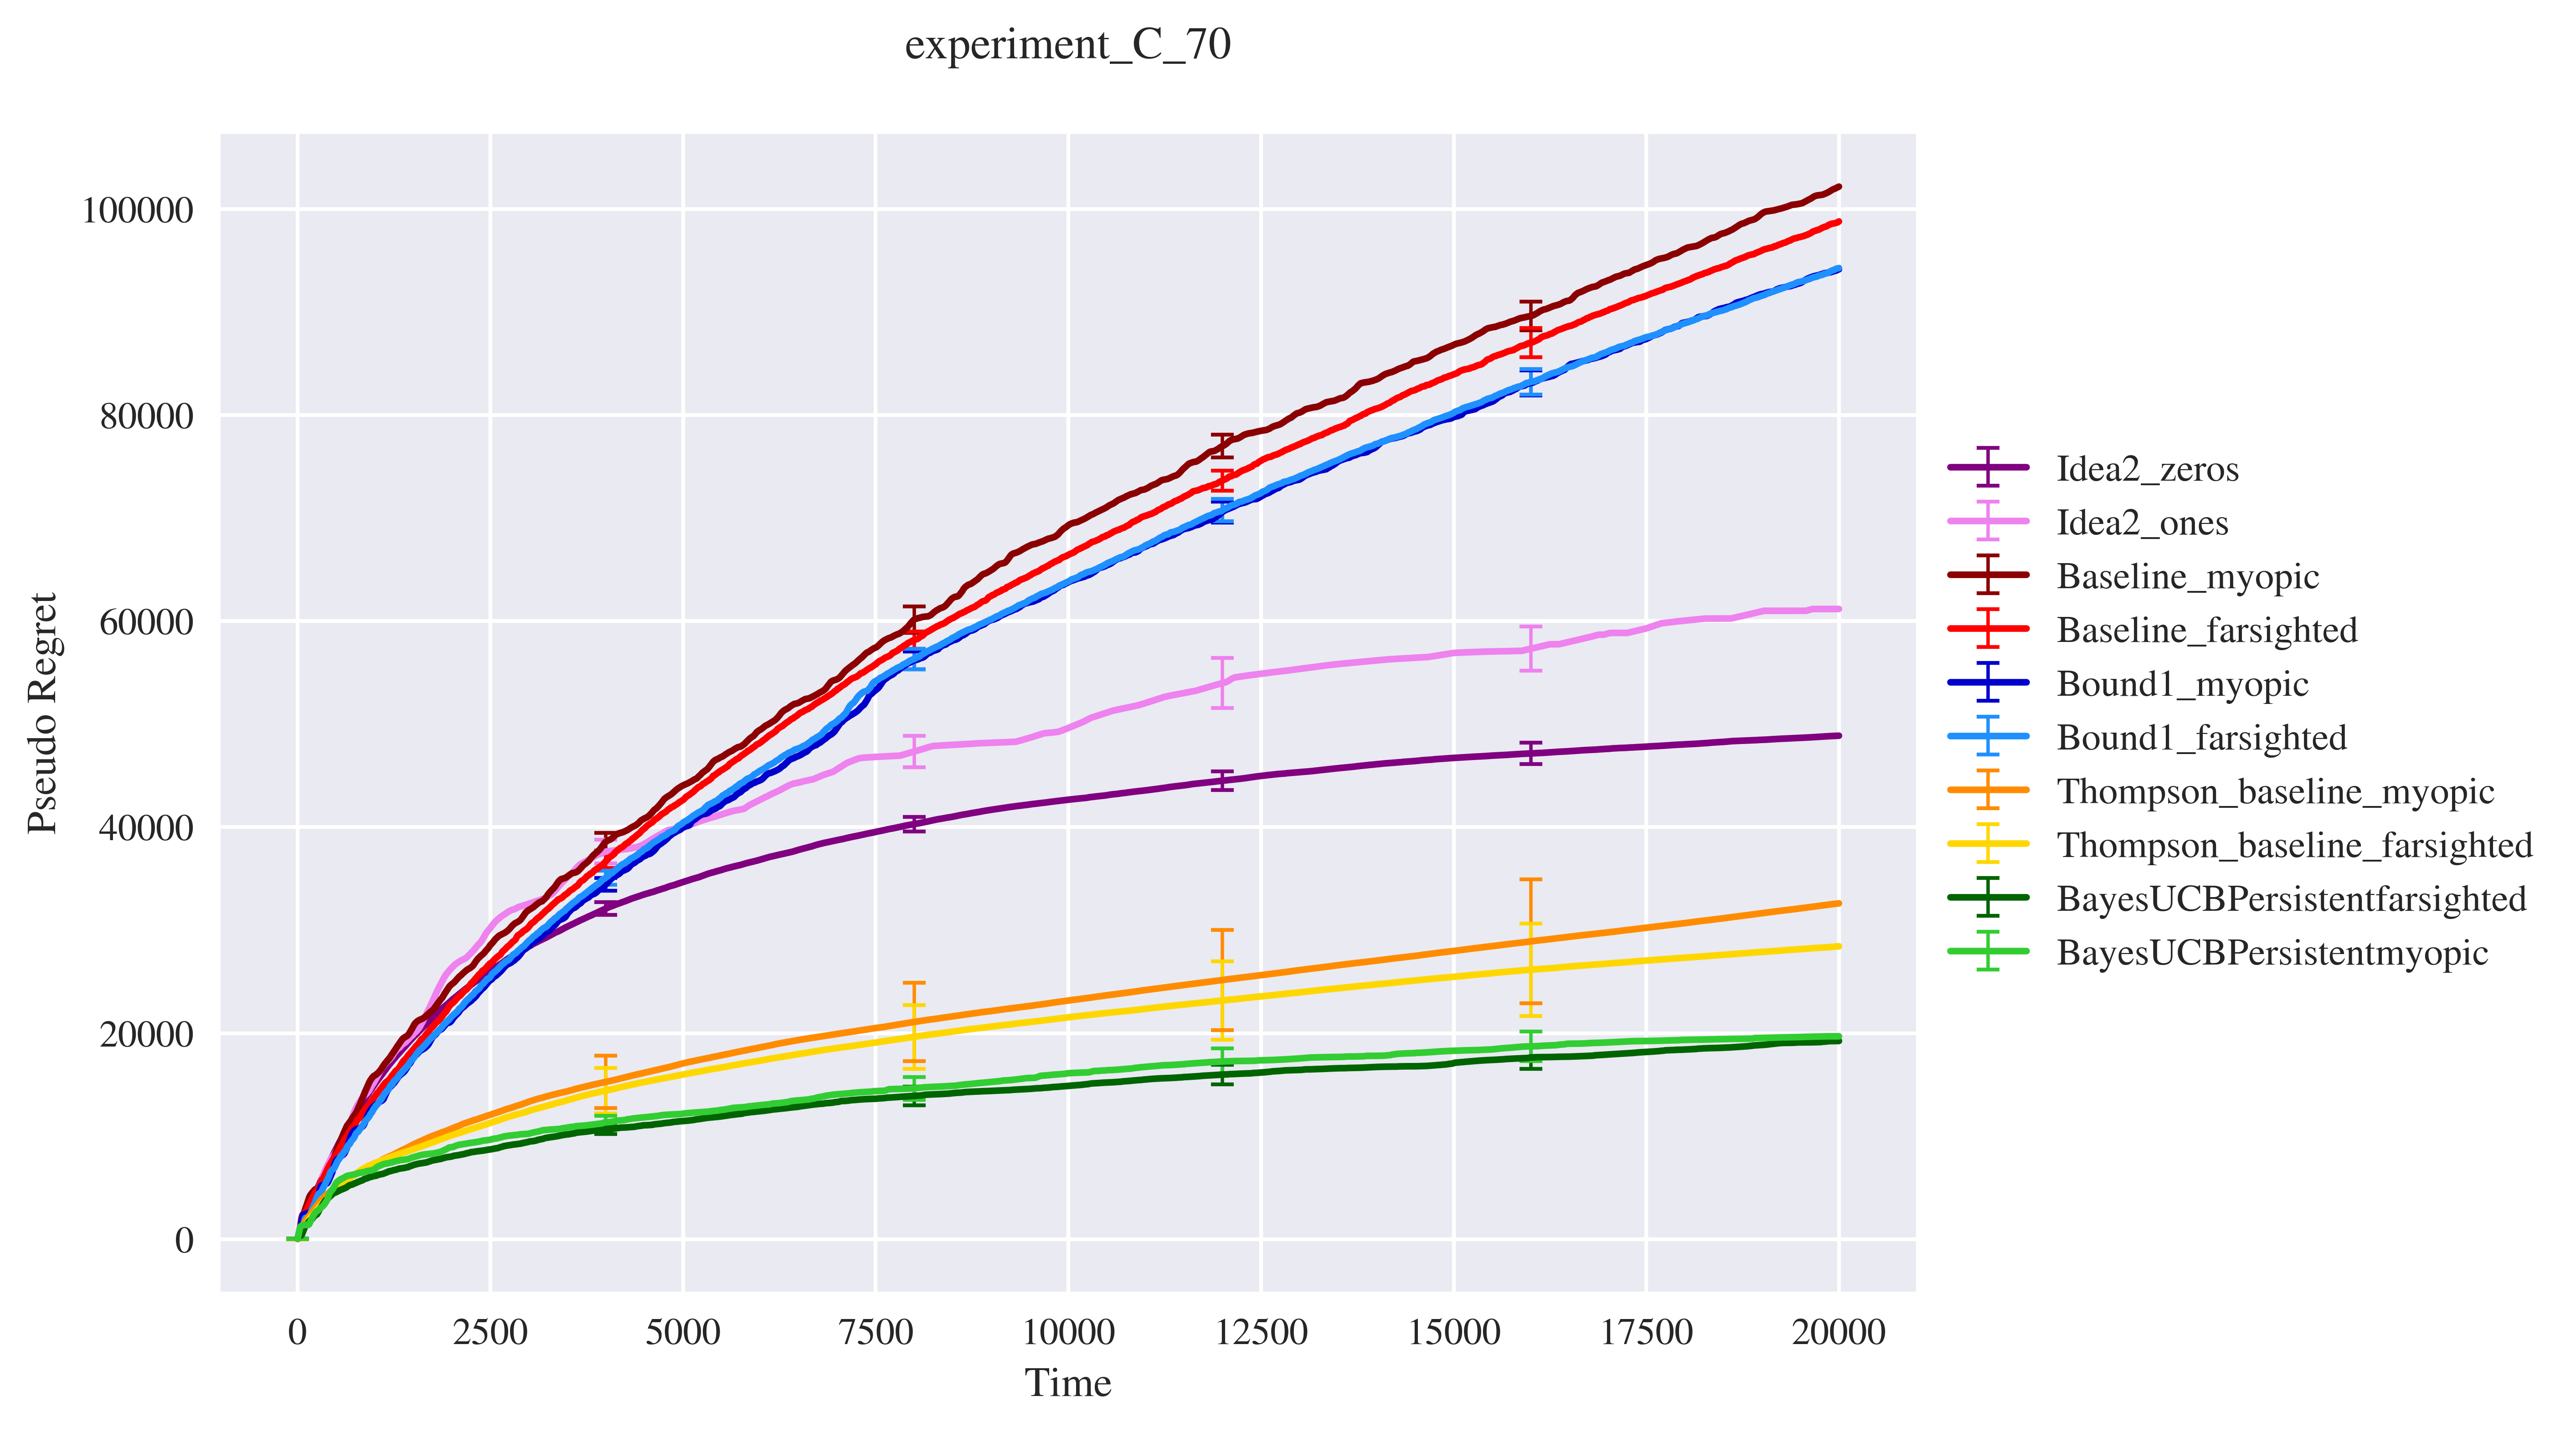
\includegraphics[width=6cm]{./images/C/experiment_C_70 ANALYTICS.png}\quad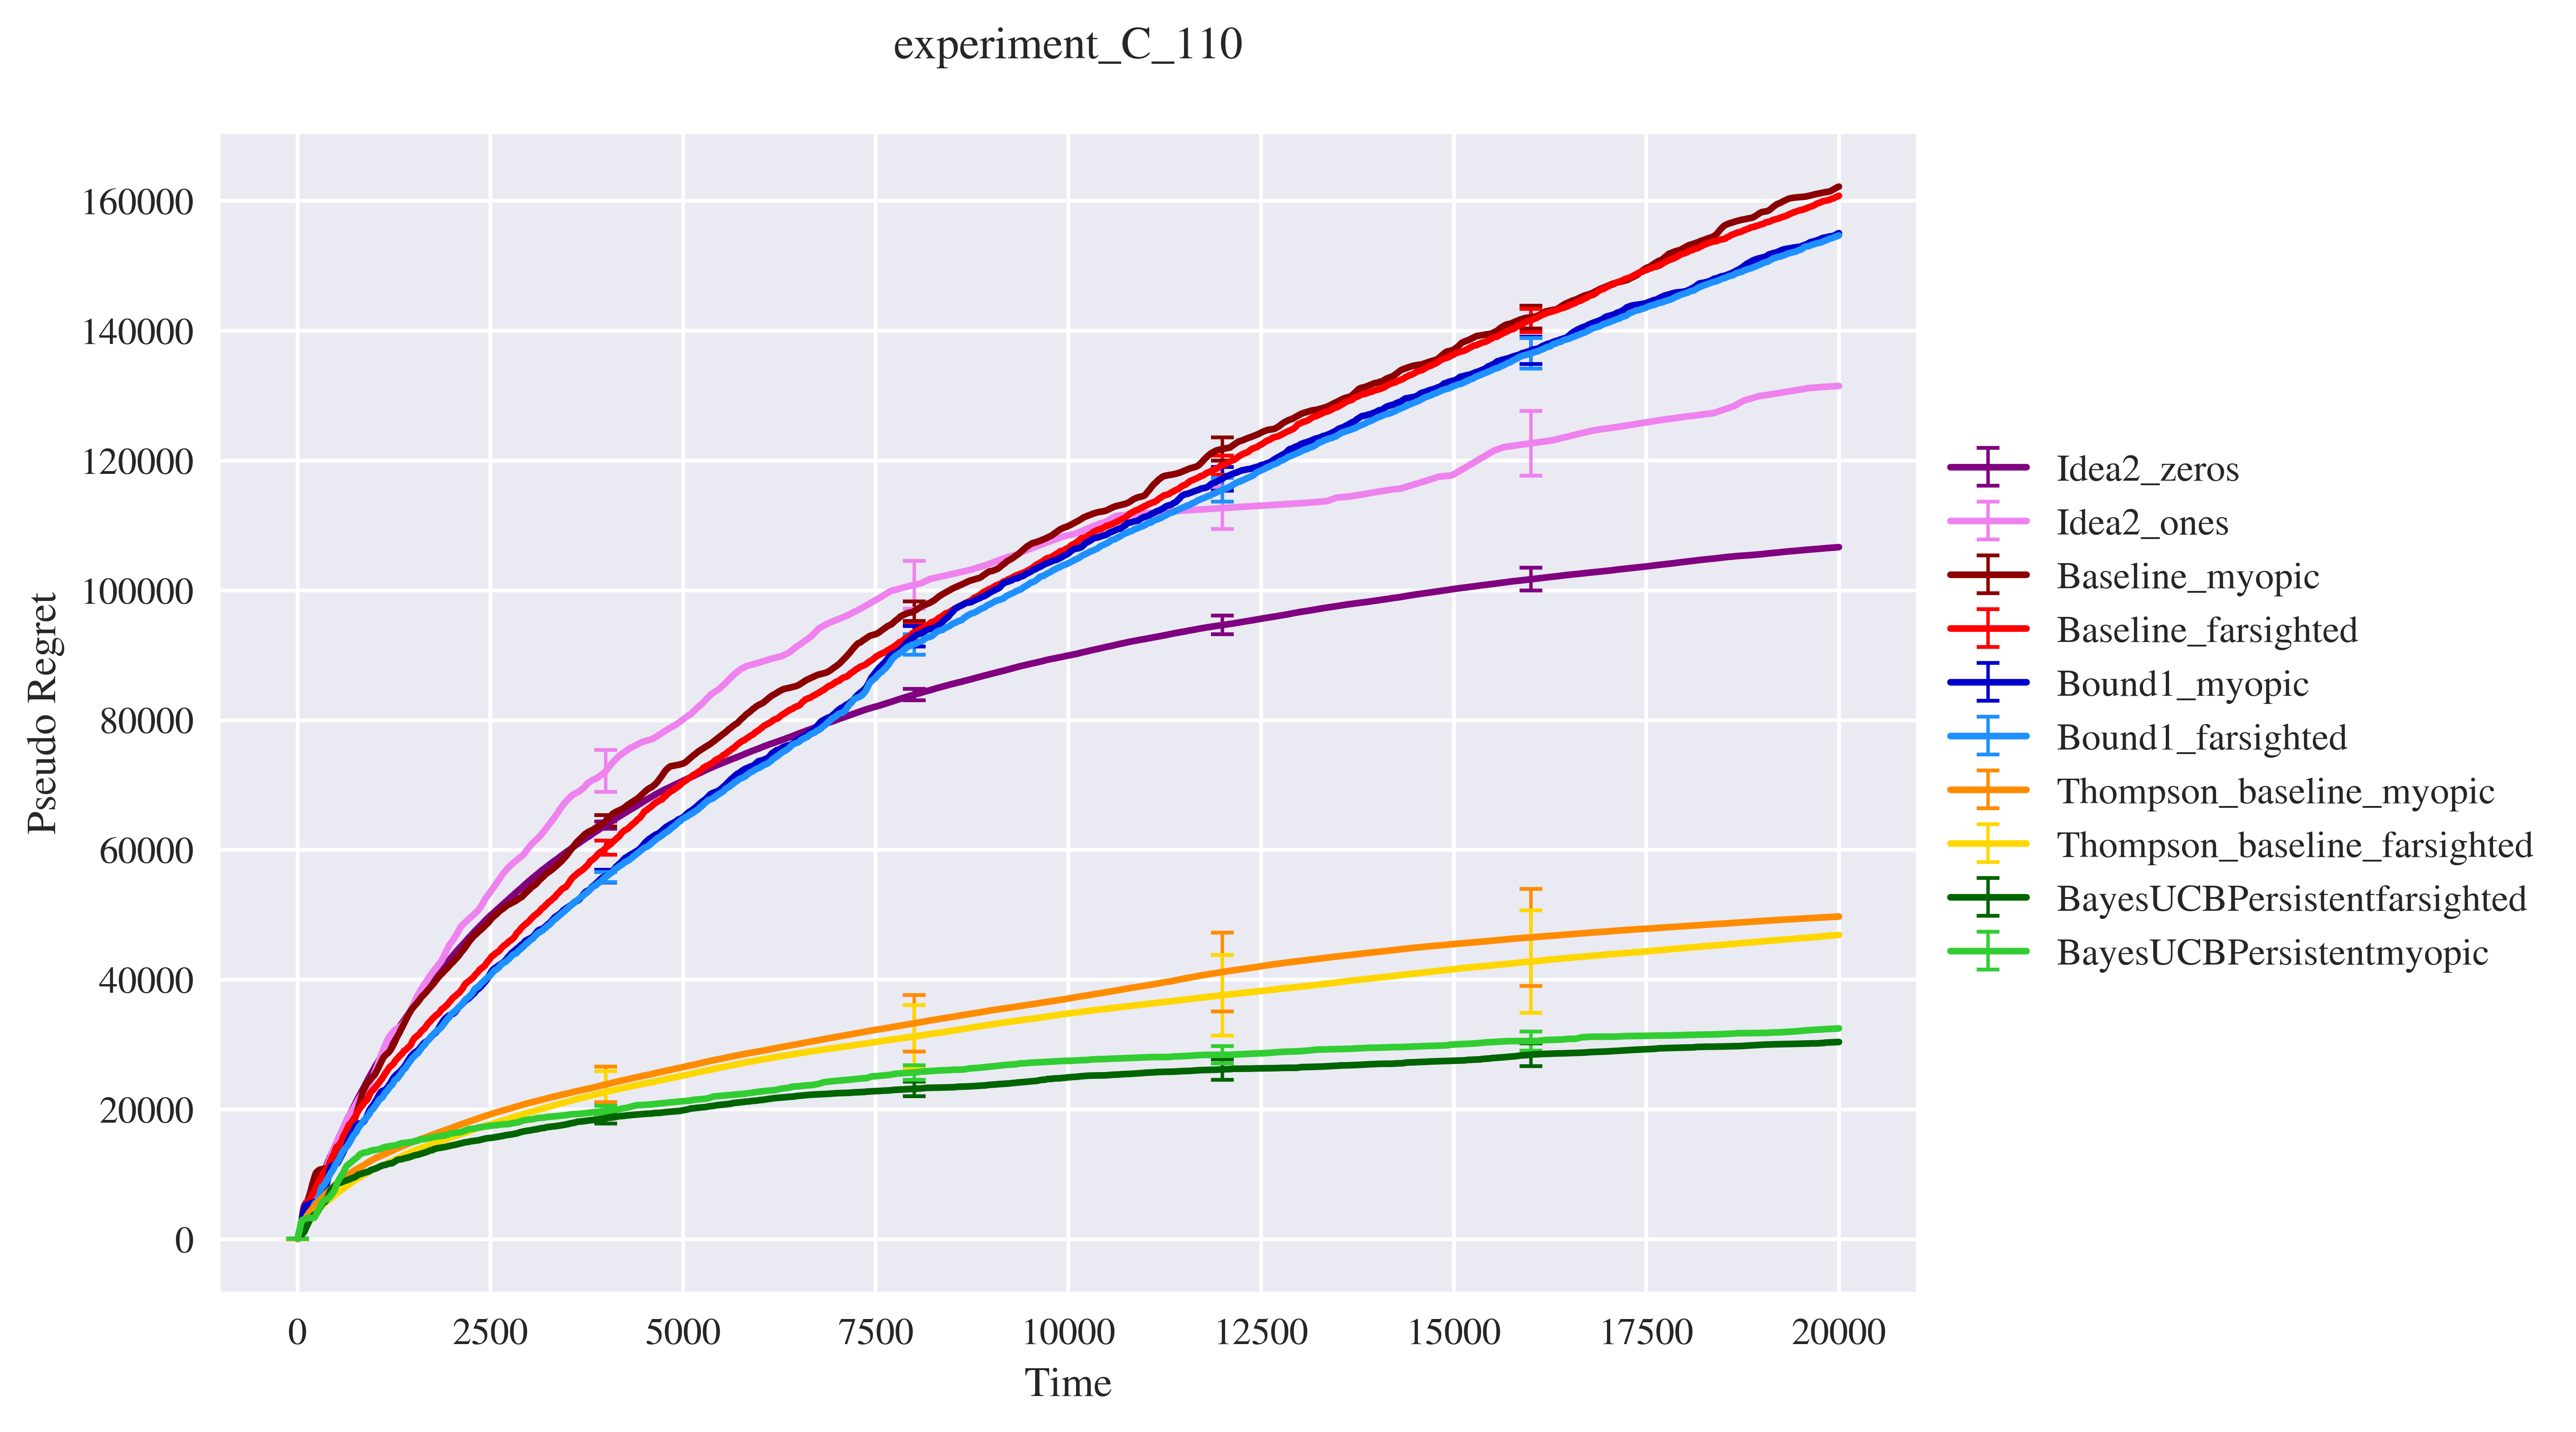
\includegraphics[width=6cm]{./images/C/experiment_C_110 ANALYTICS.png}
	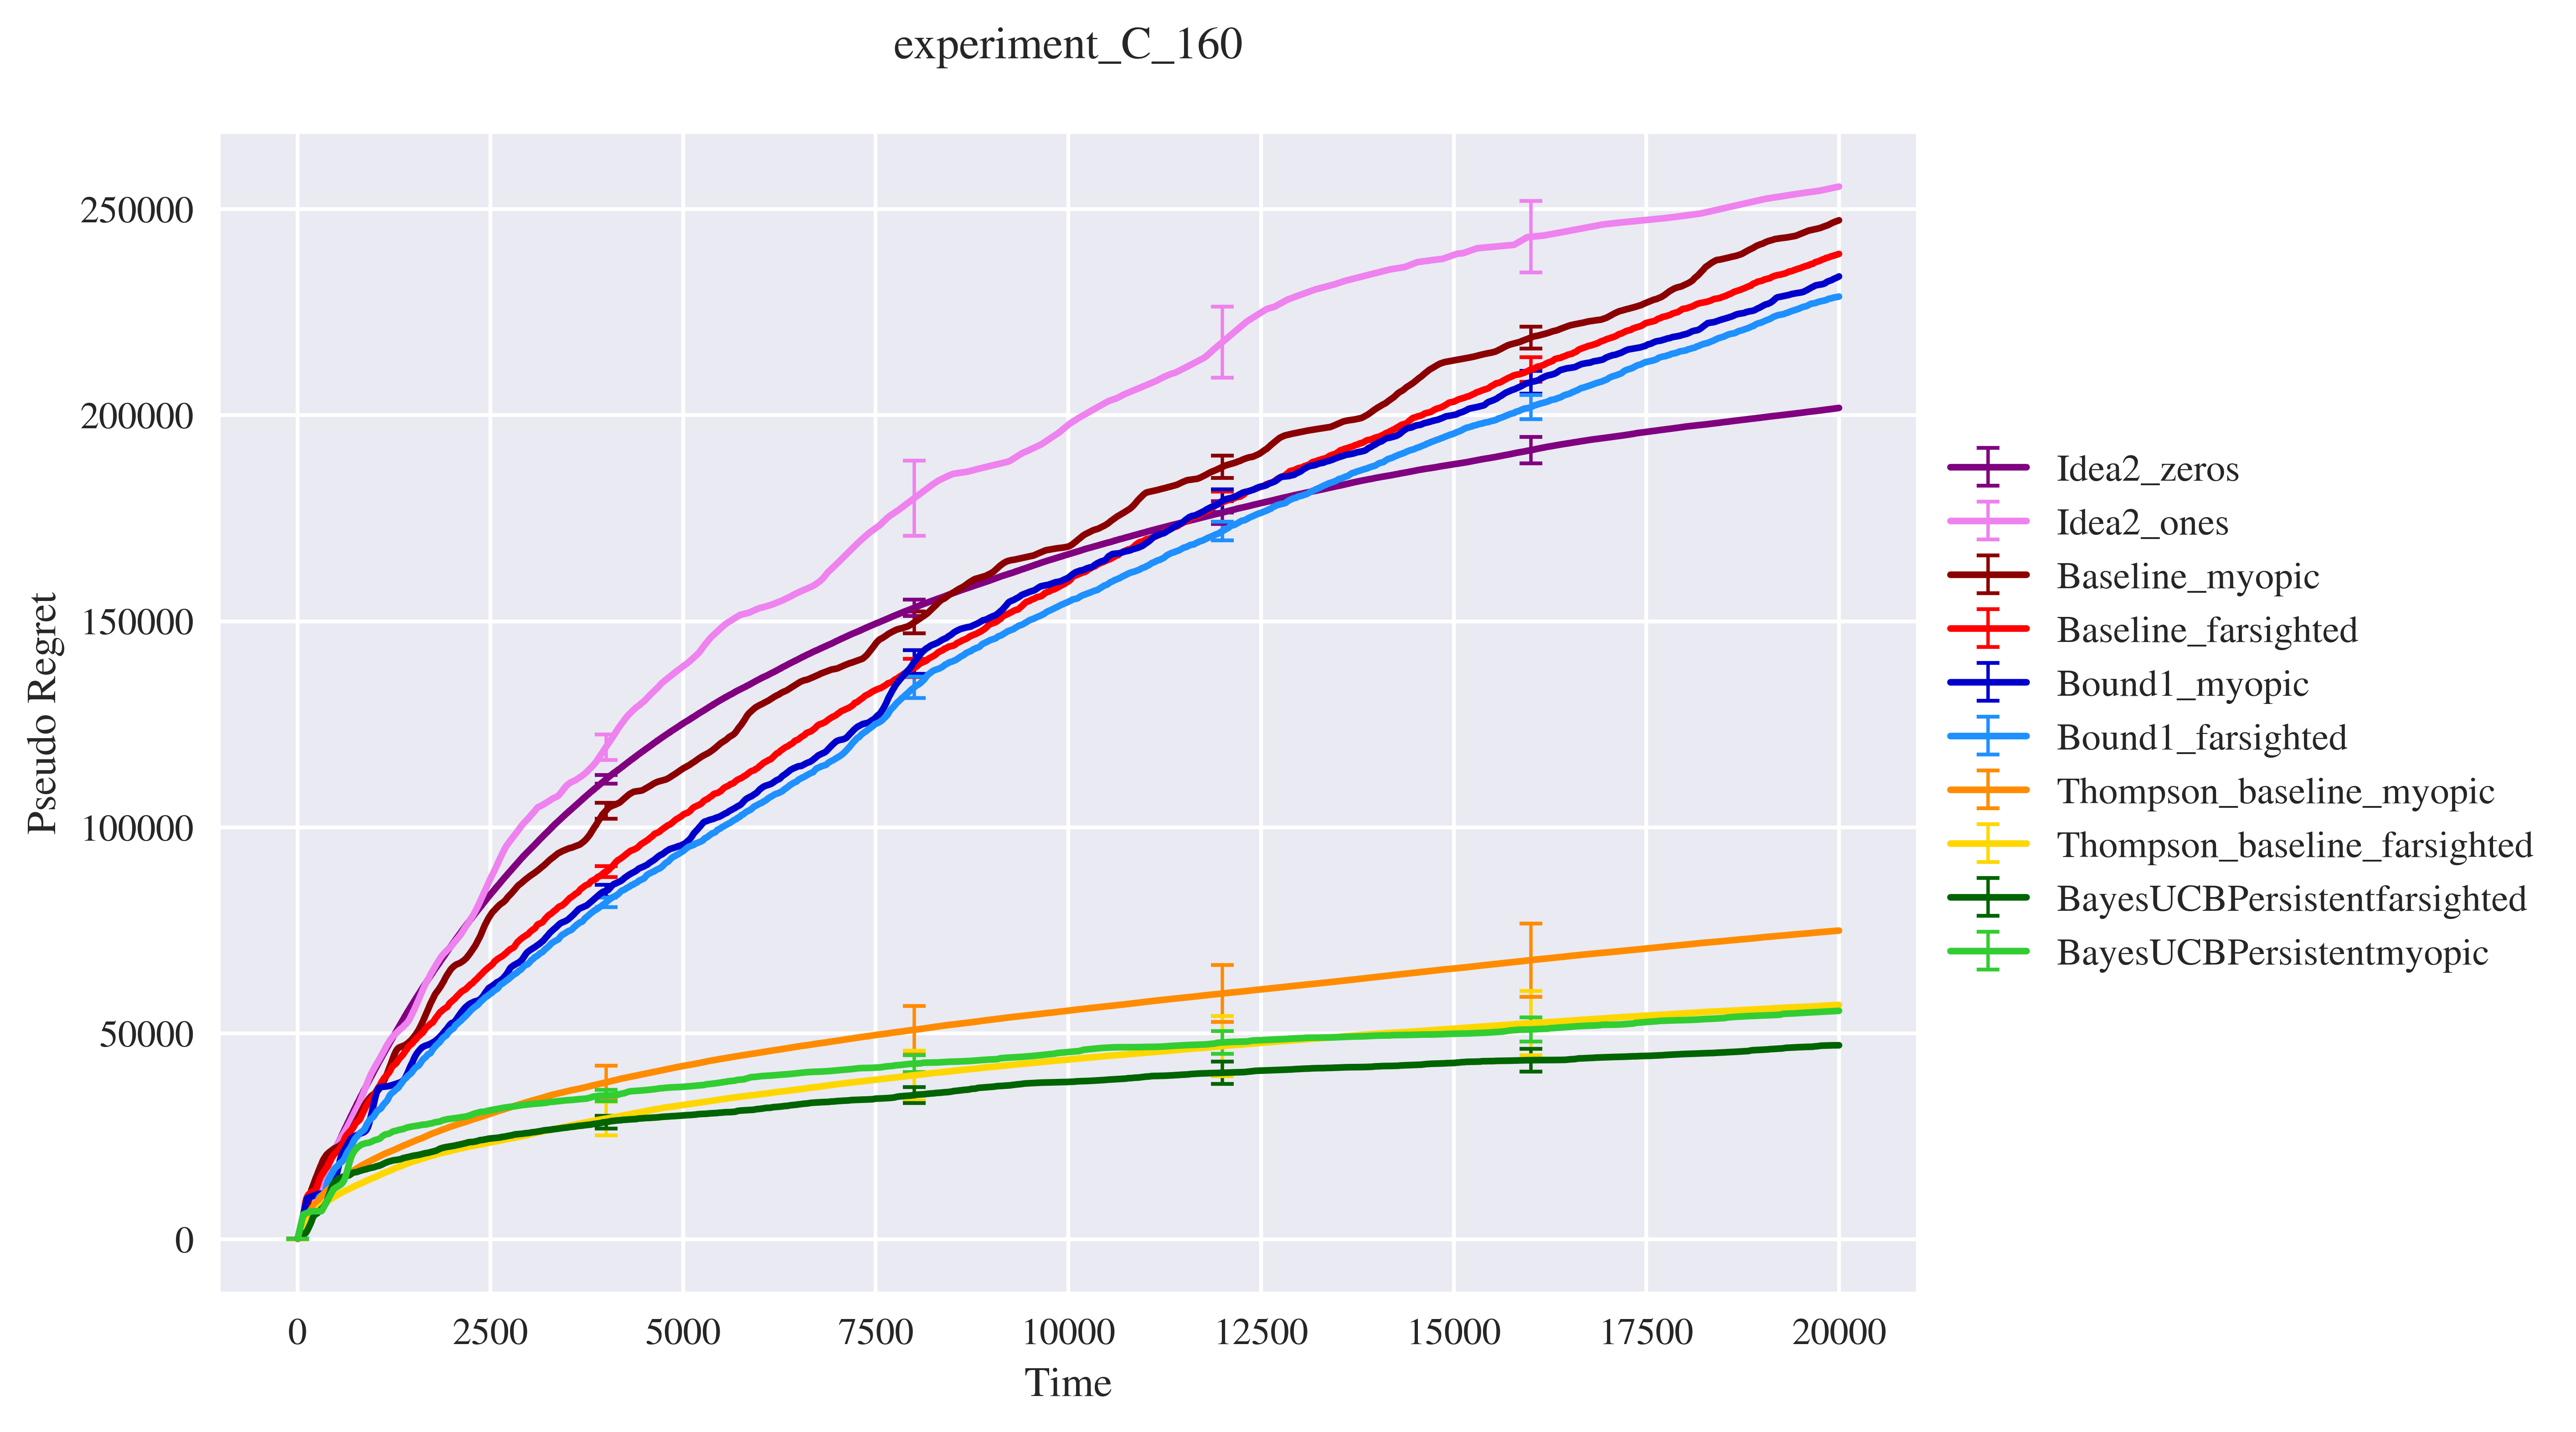
\includegraphics[width=6cm]{./images/C/experiment_C_160 ANALYTICS.png}\quad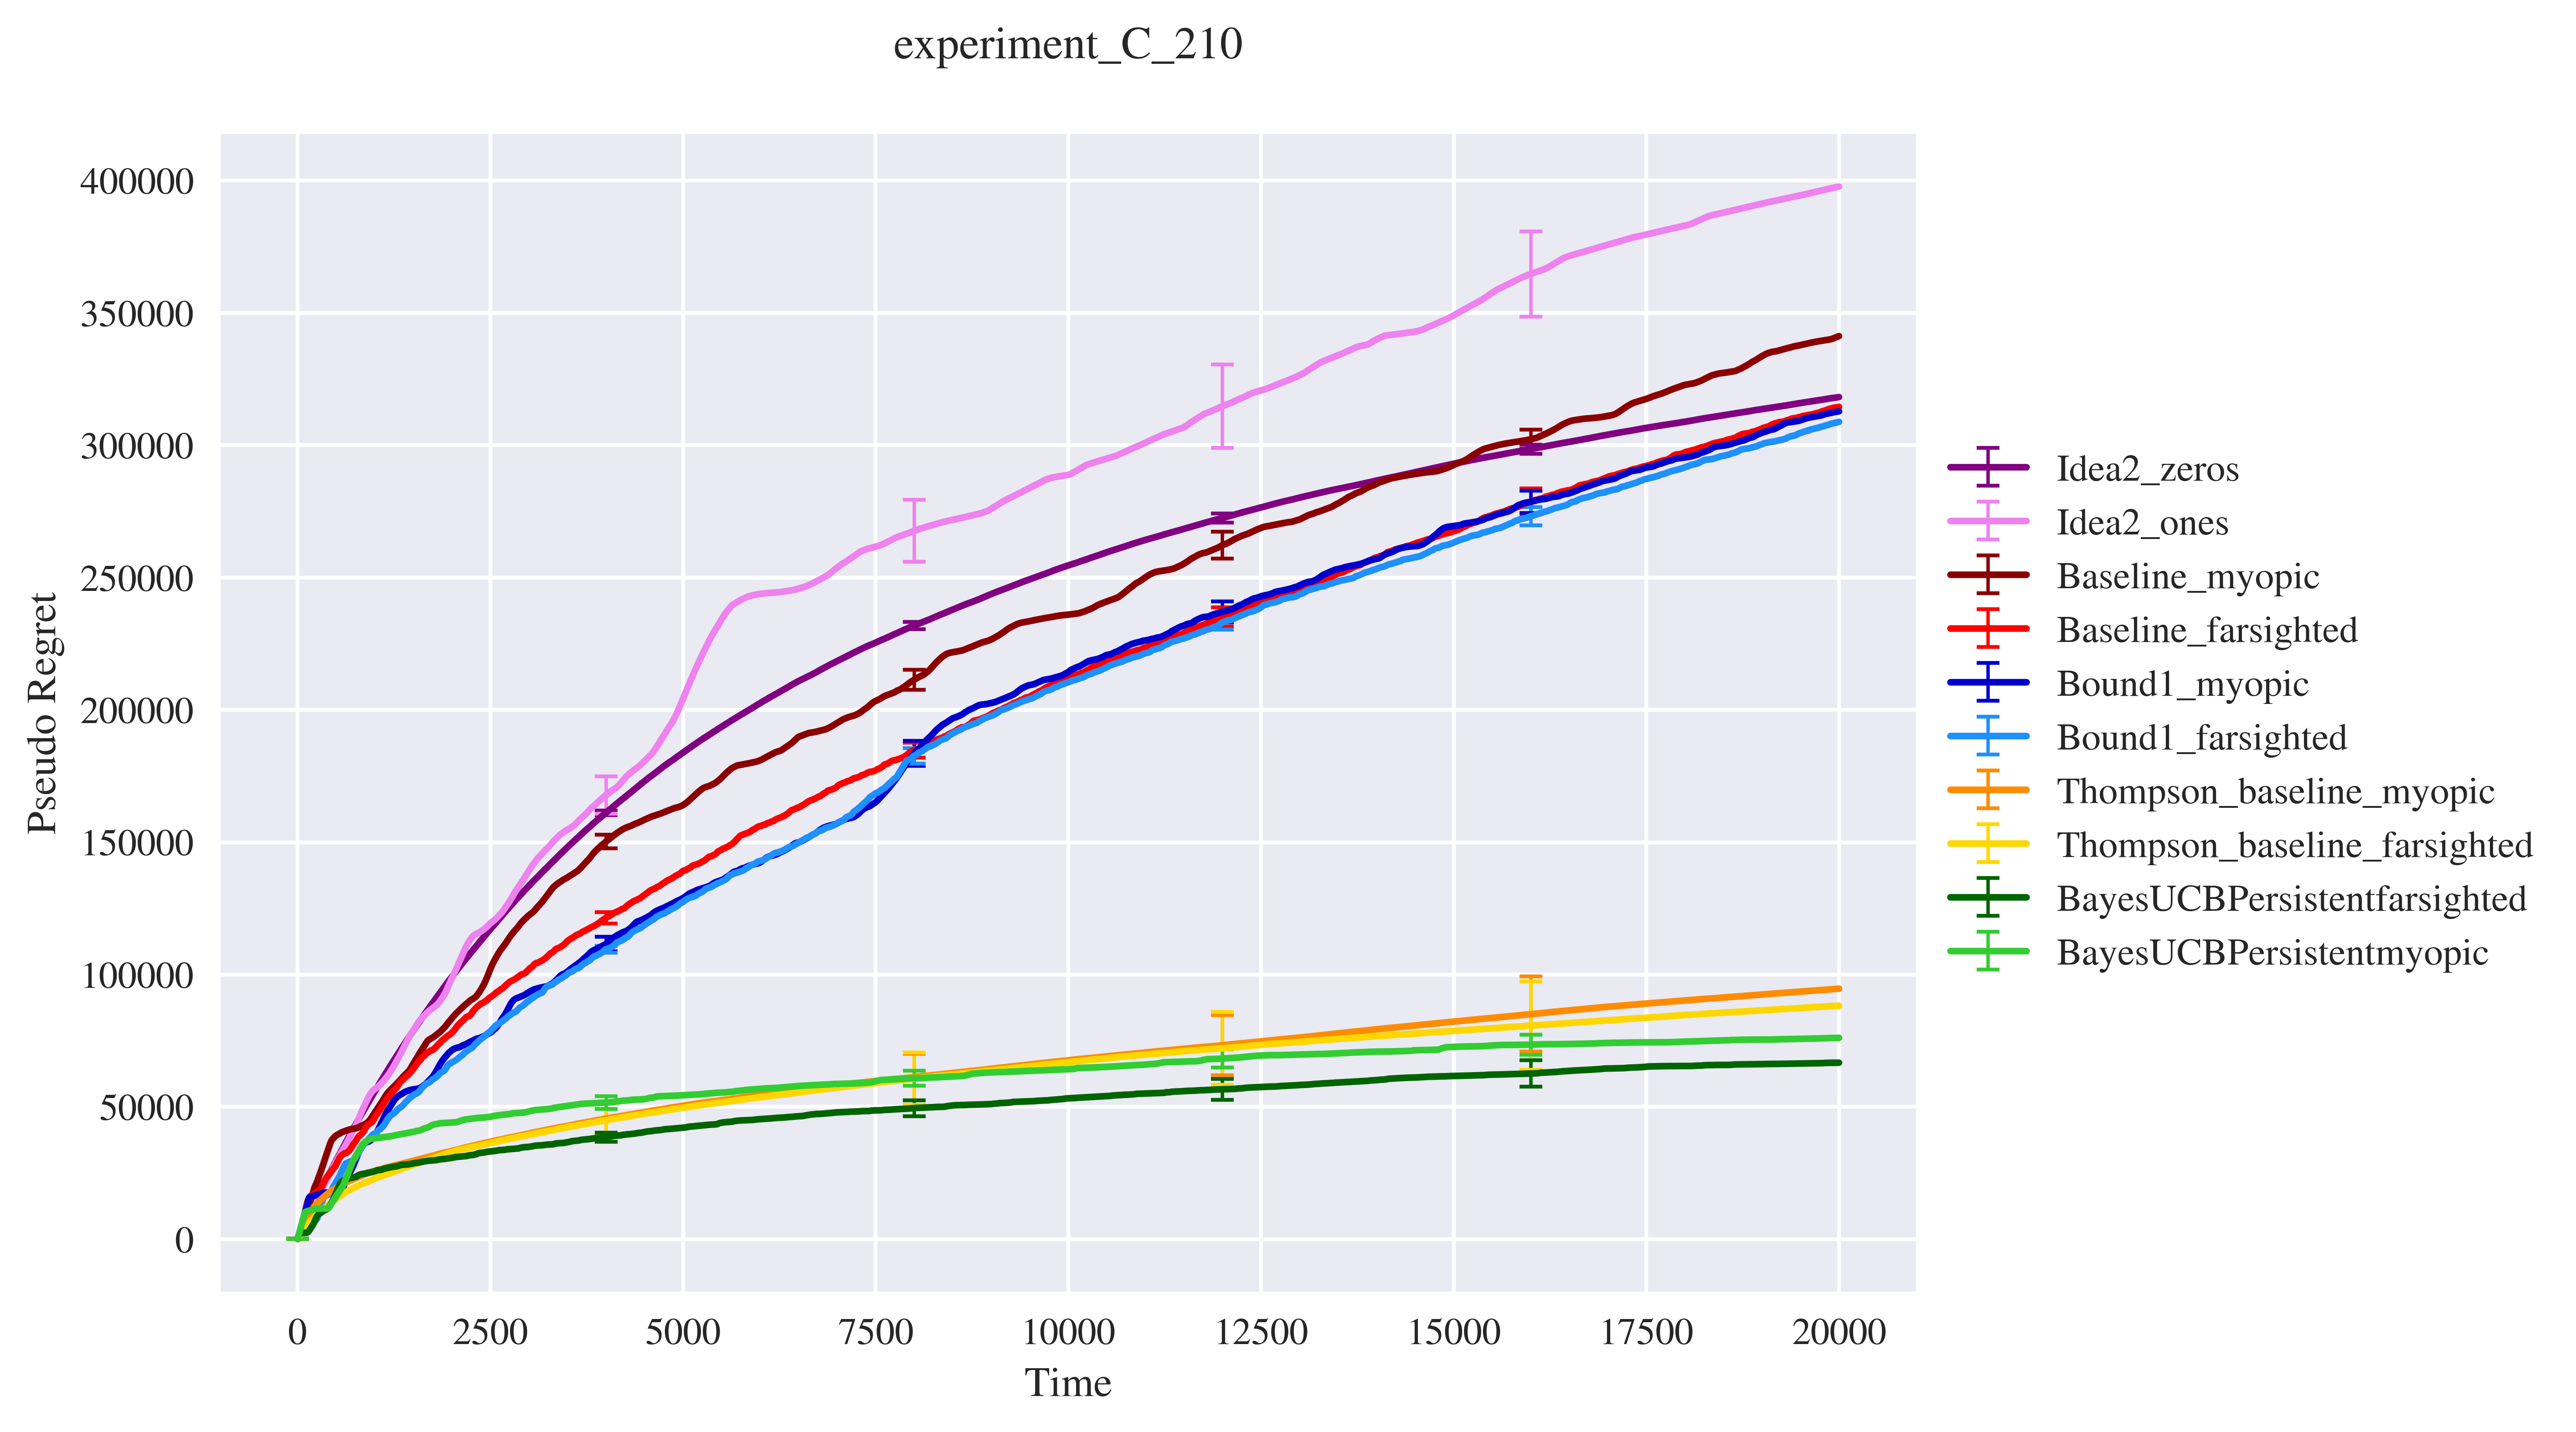
\includegraphics[width=6cm]{./images/C/experiment_C_210 ANALYTICS.png}
	\caption{SYNTHETIC C}
	
\end{figure}



\begin{figure}[h]
	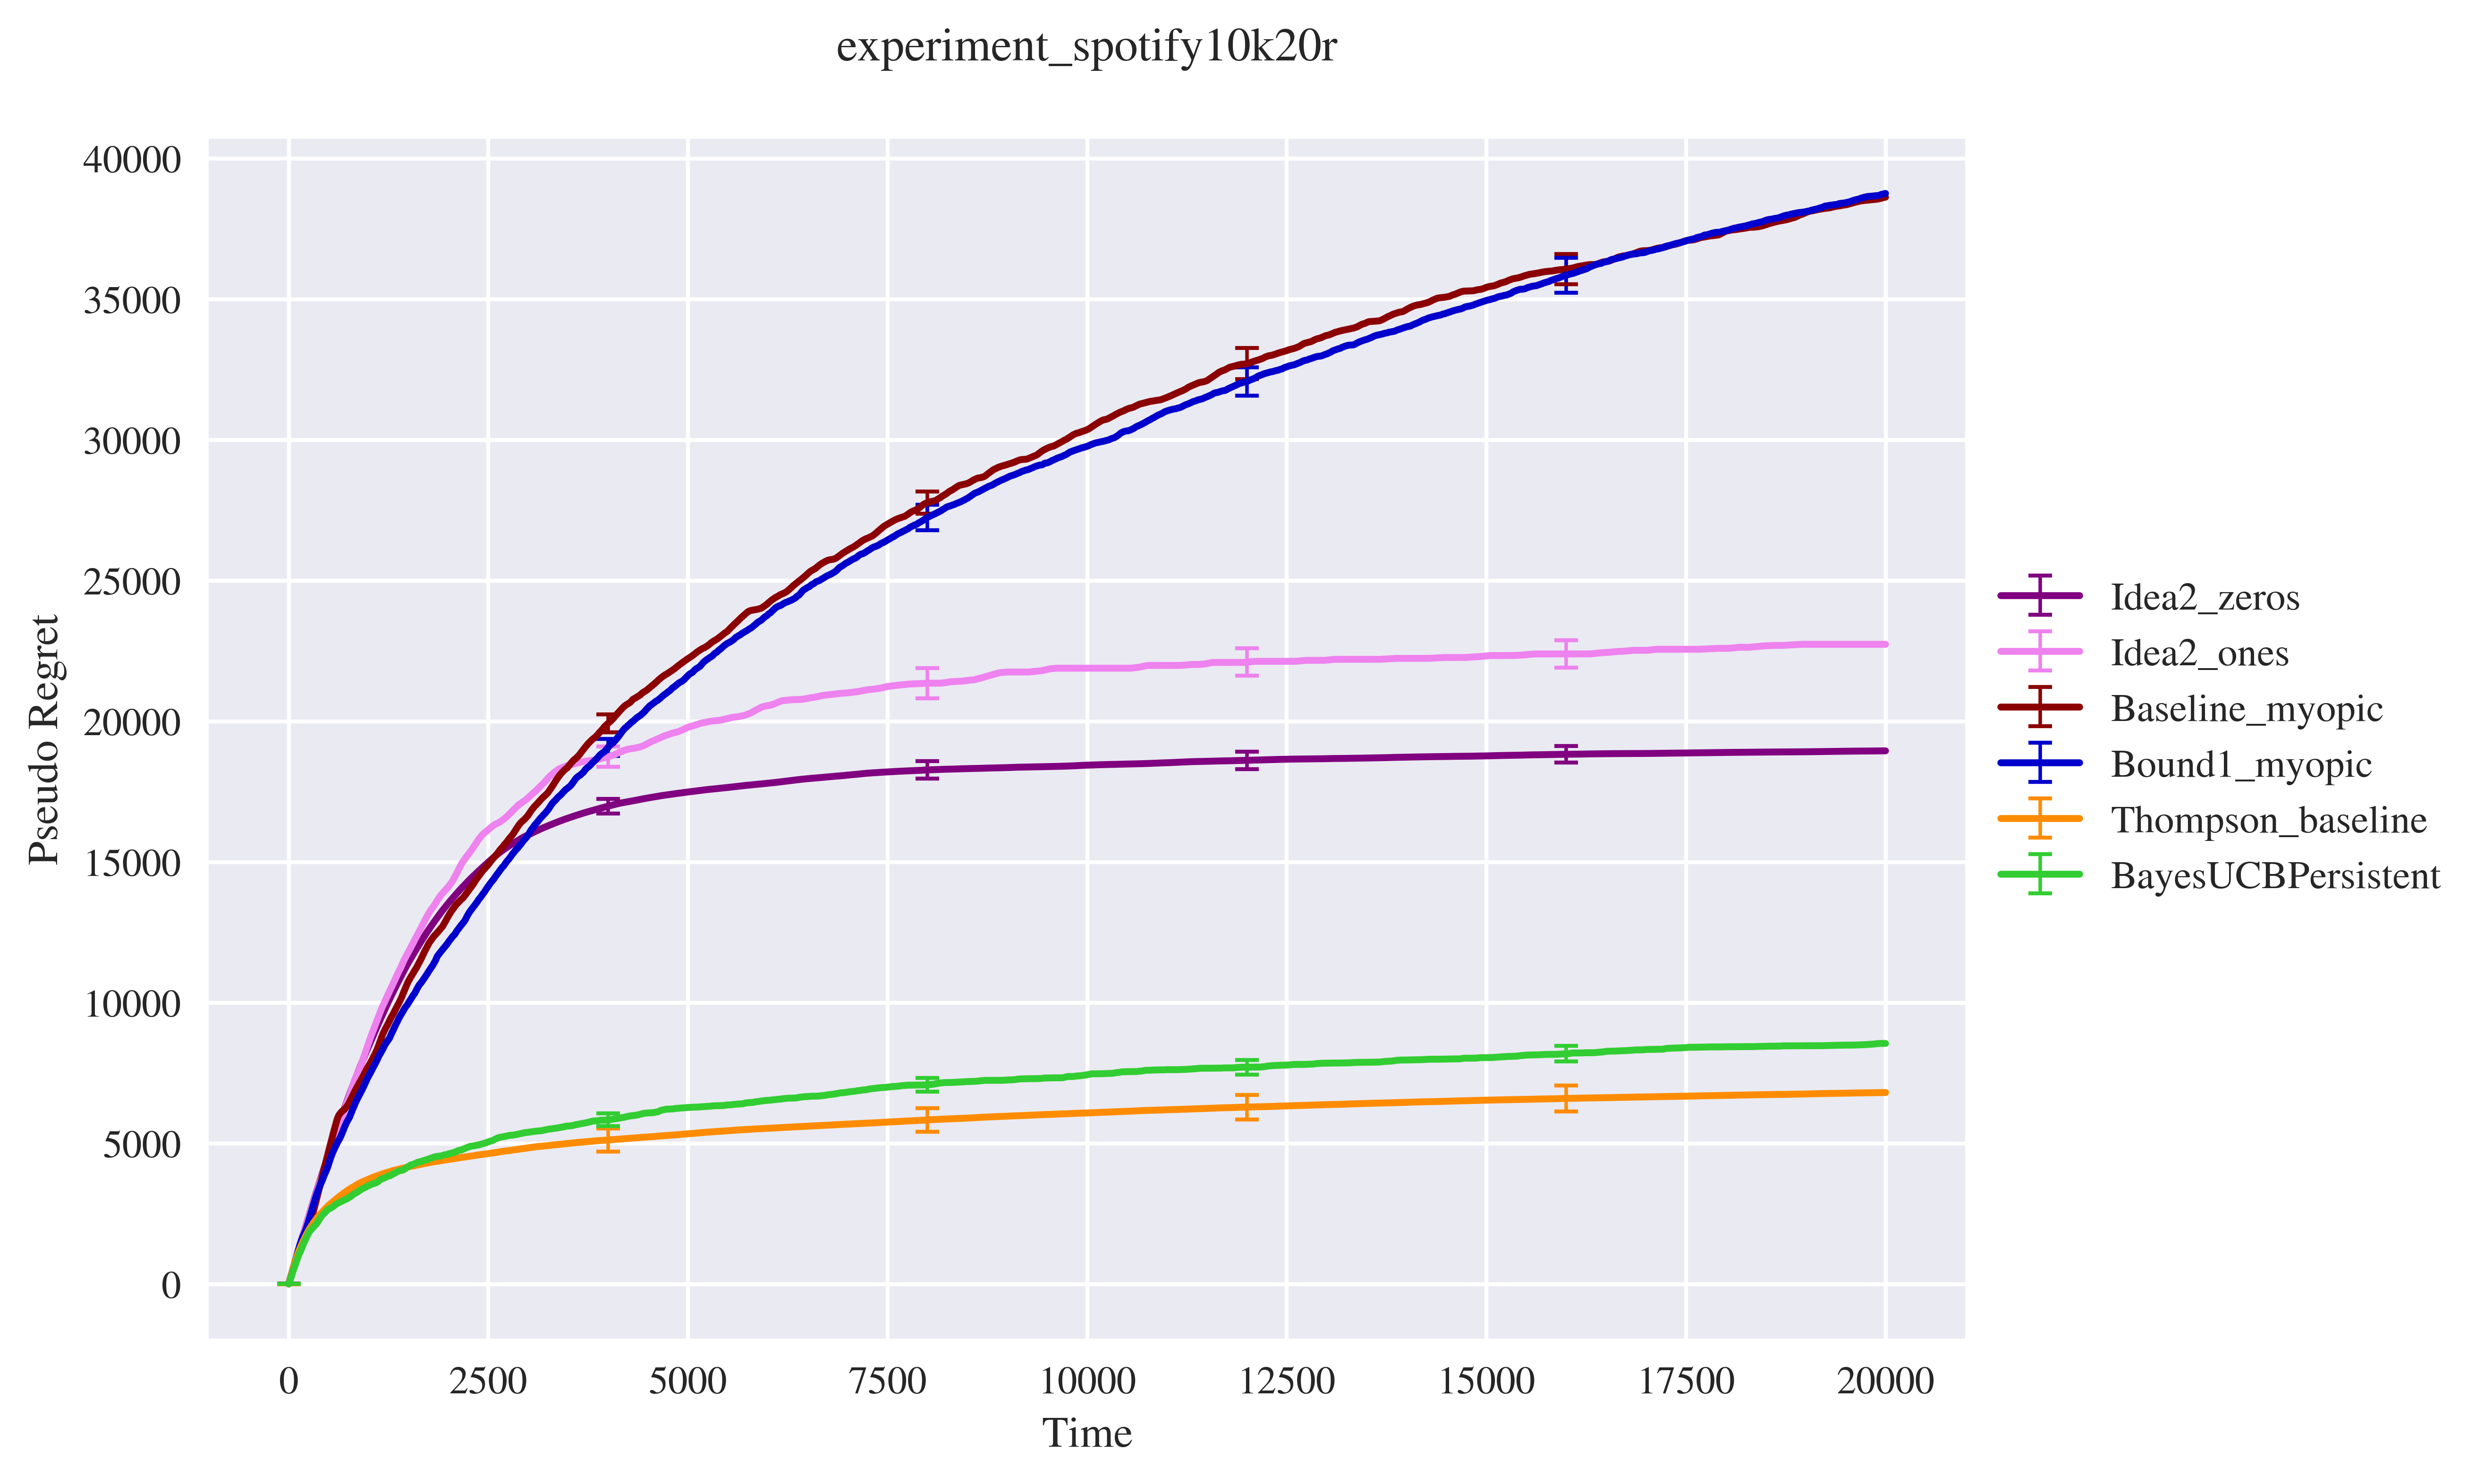
\includegraphics[width=16cm]{./images/experiment_spotify10k20r ANALYTICS.png}
	\centering	
	\caption{Spotify Scenario}
\end{figure}


\begin{figure}
	\centering
	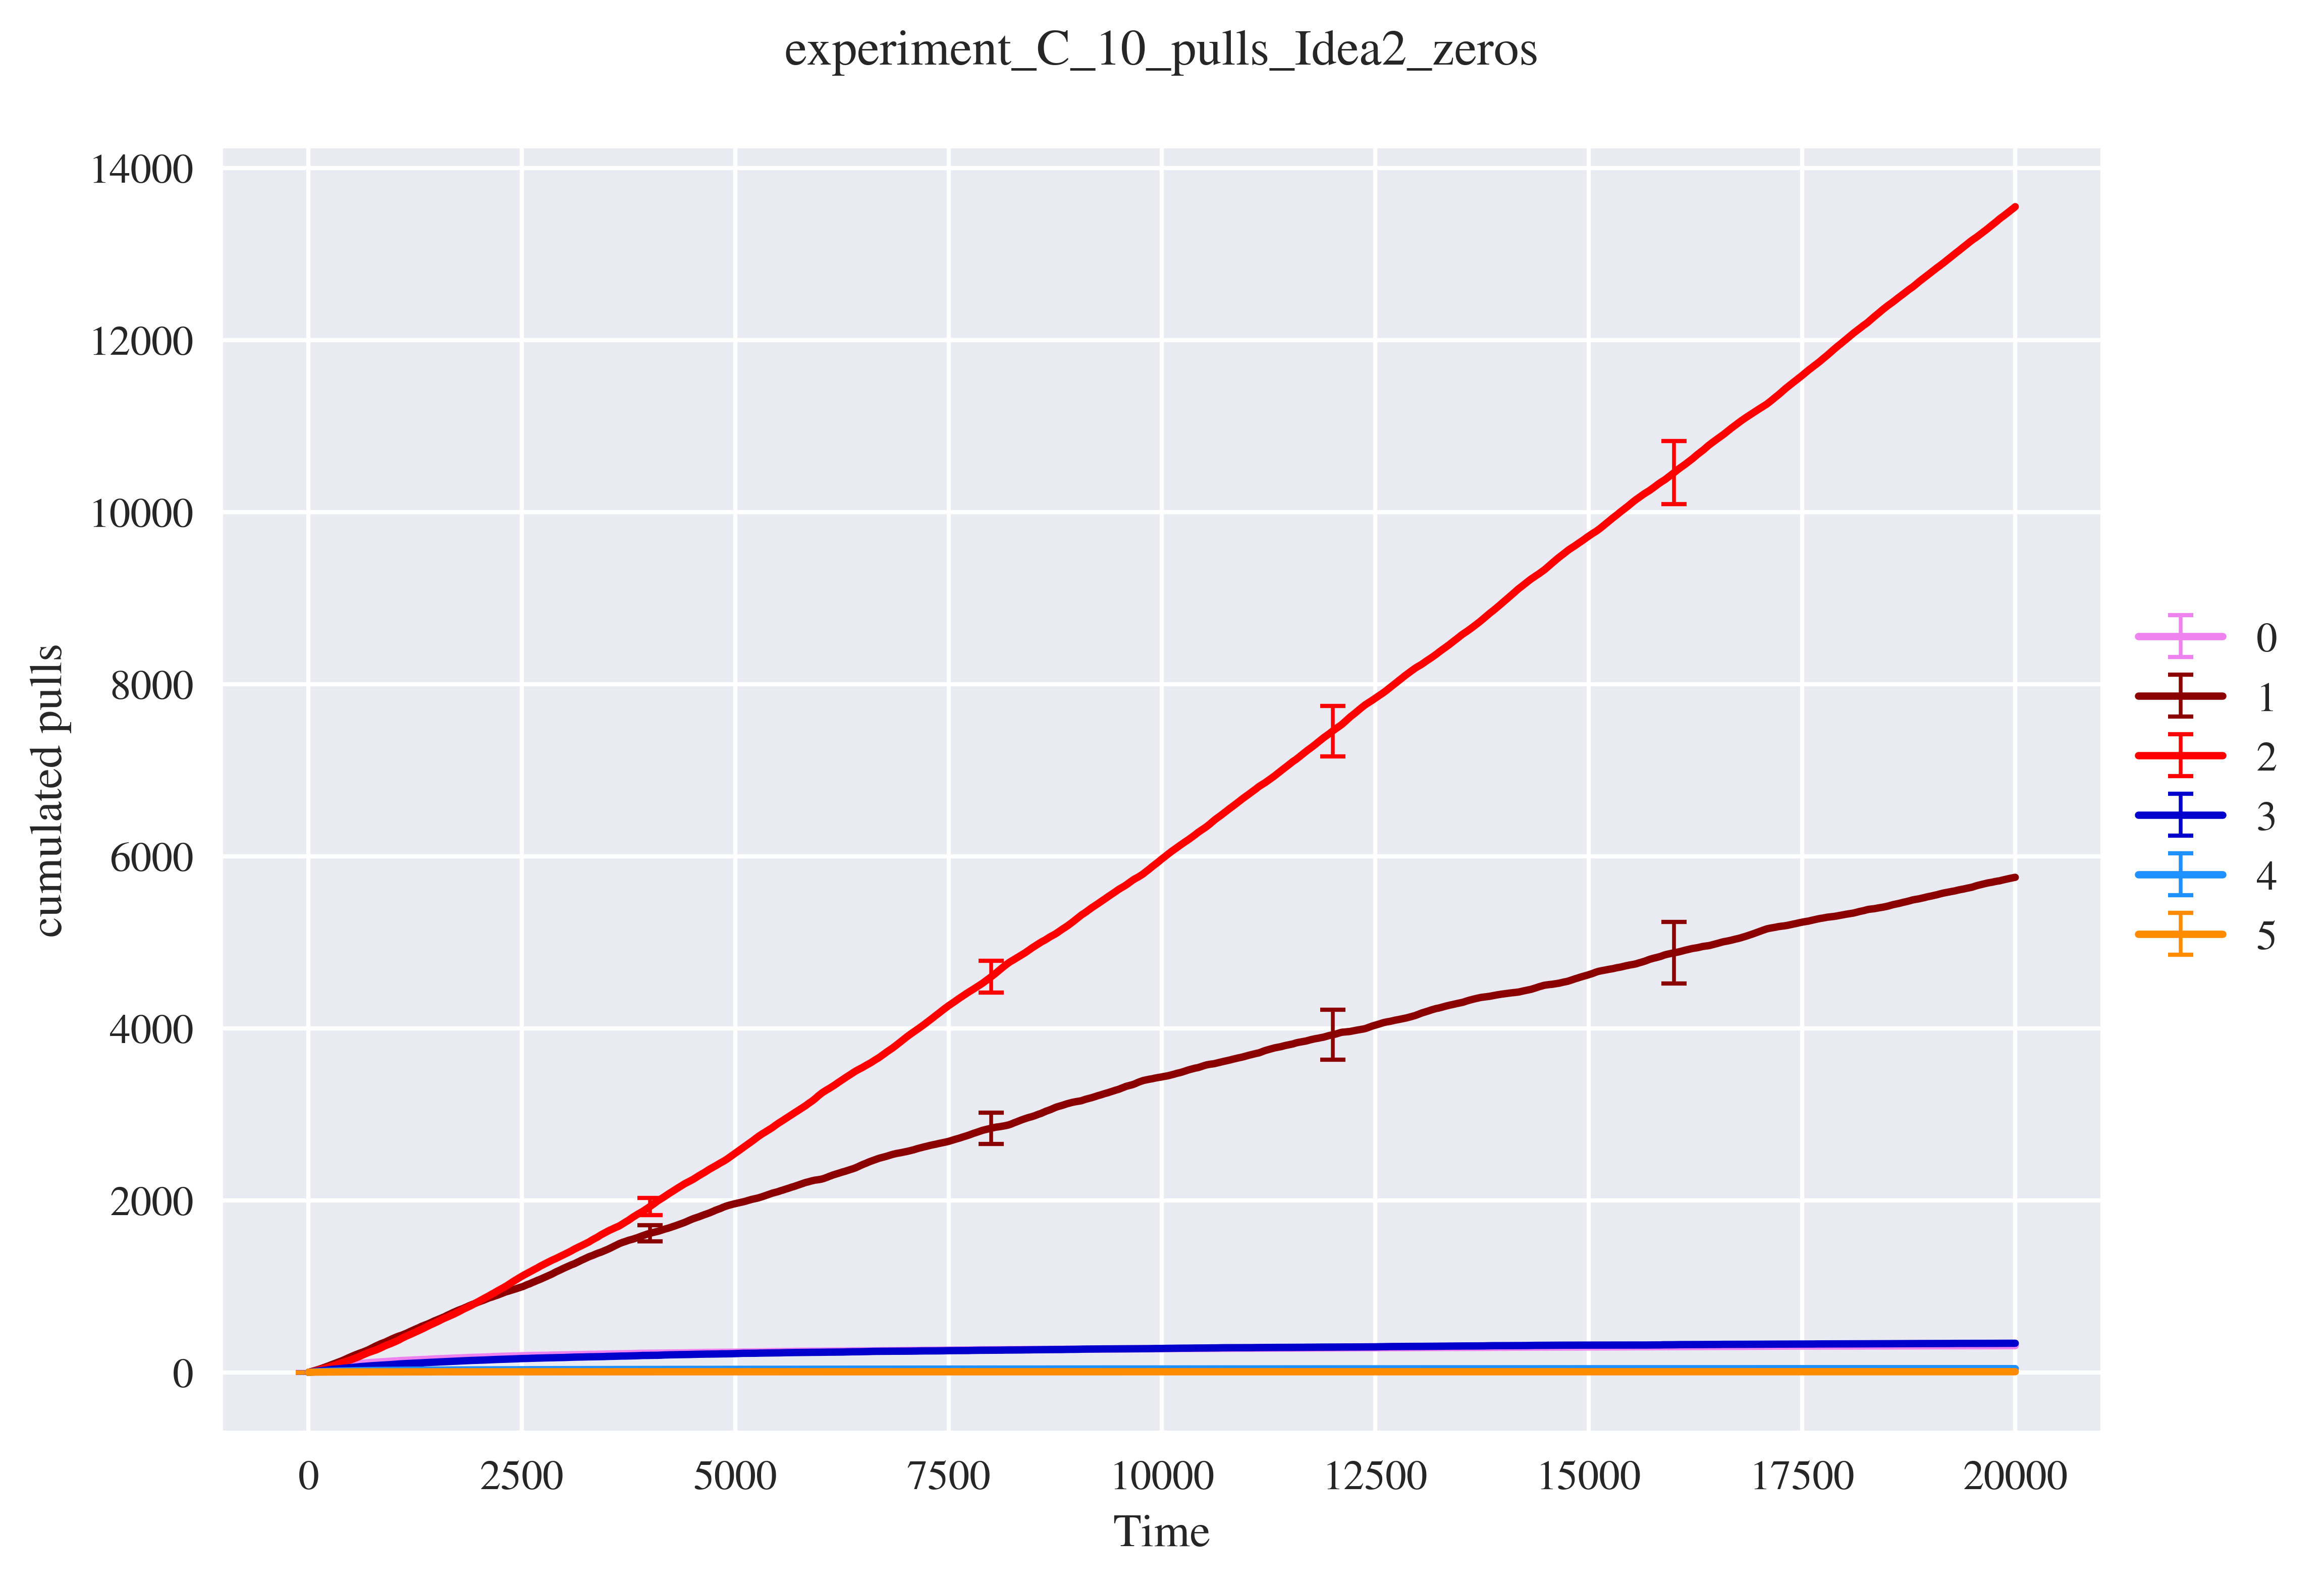
\includegraphics[width=6cm]{./images/PULLS/experiment_C_10Idea2_zeros cum_pulls.png }\quad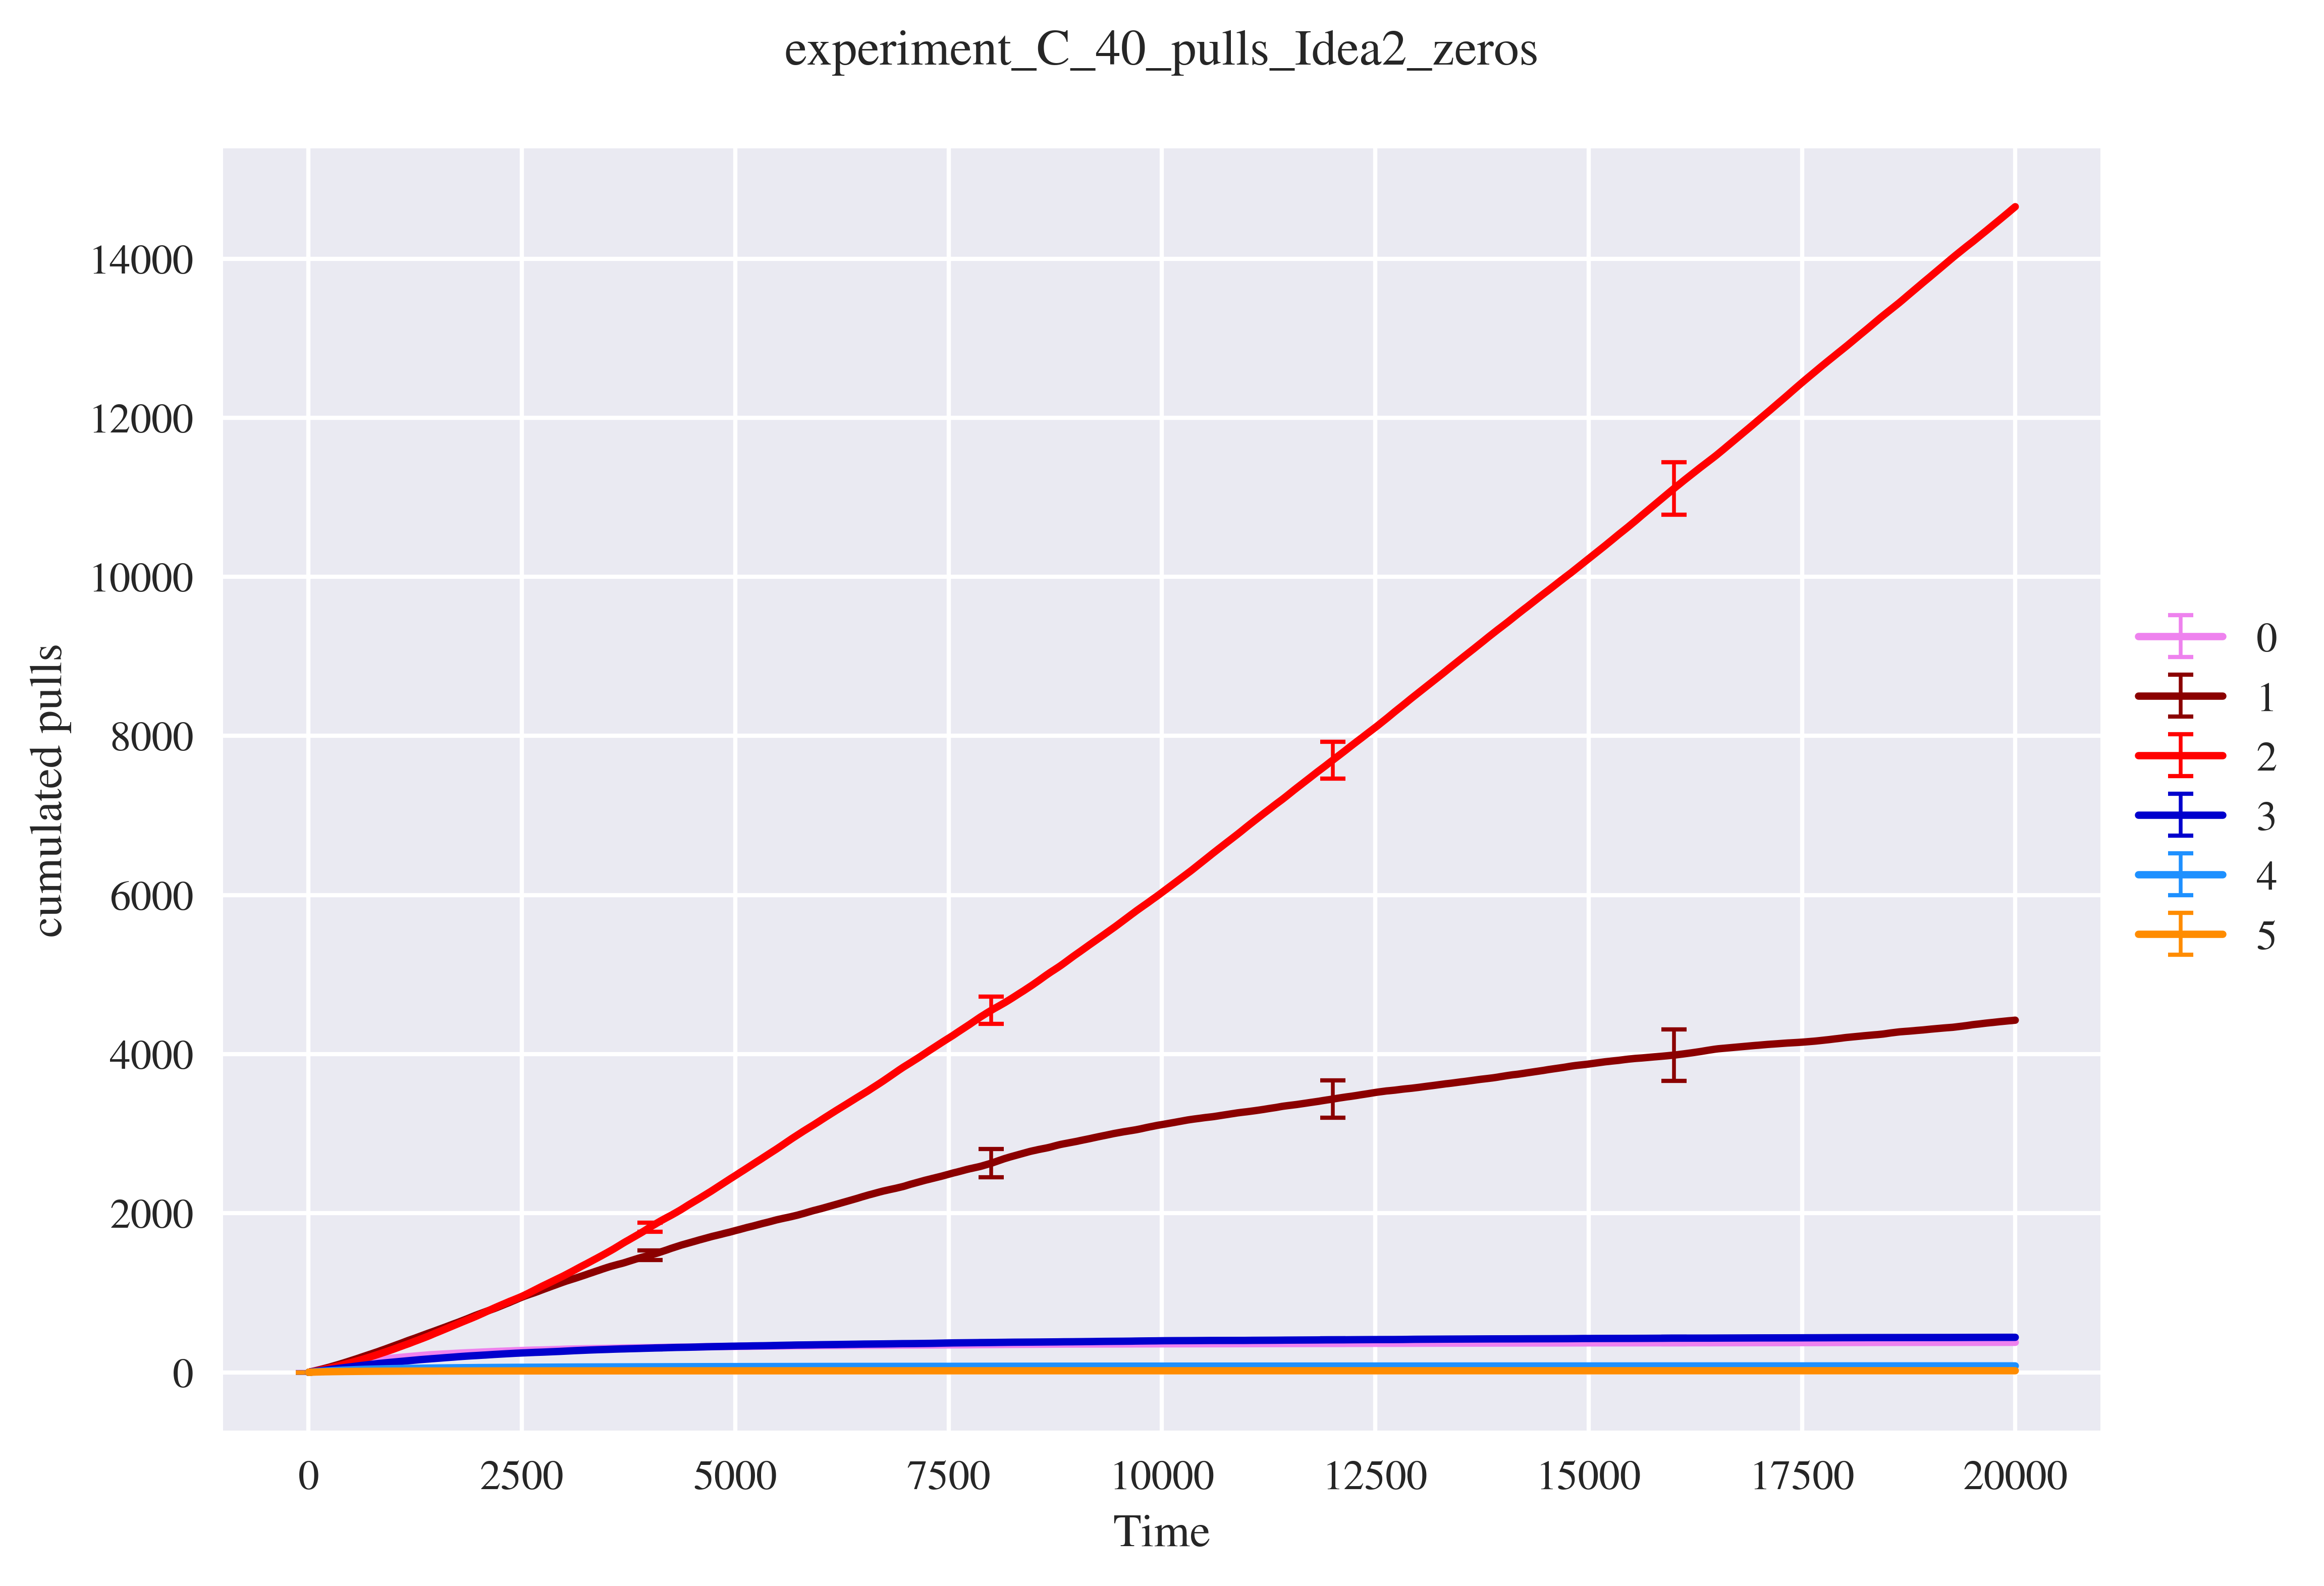
\includegraphics[width=6cm]{./images/PULLS/experiment_C_40Idea2_zeros cum_pulls.png
	} 
	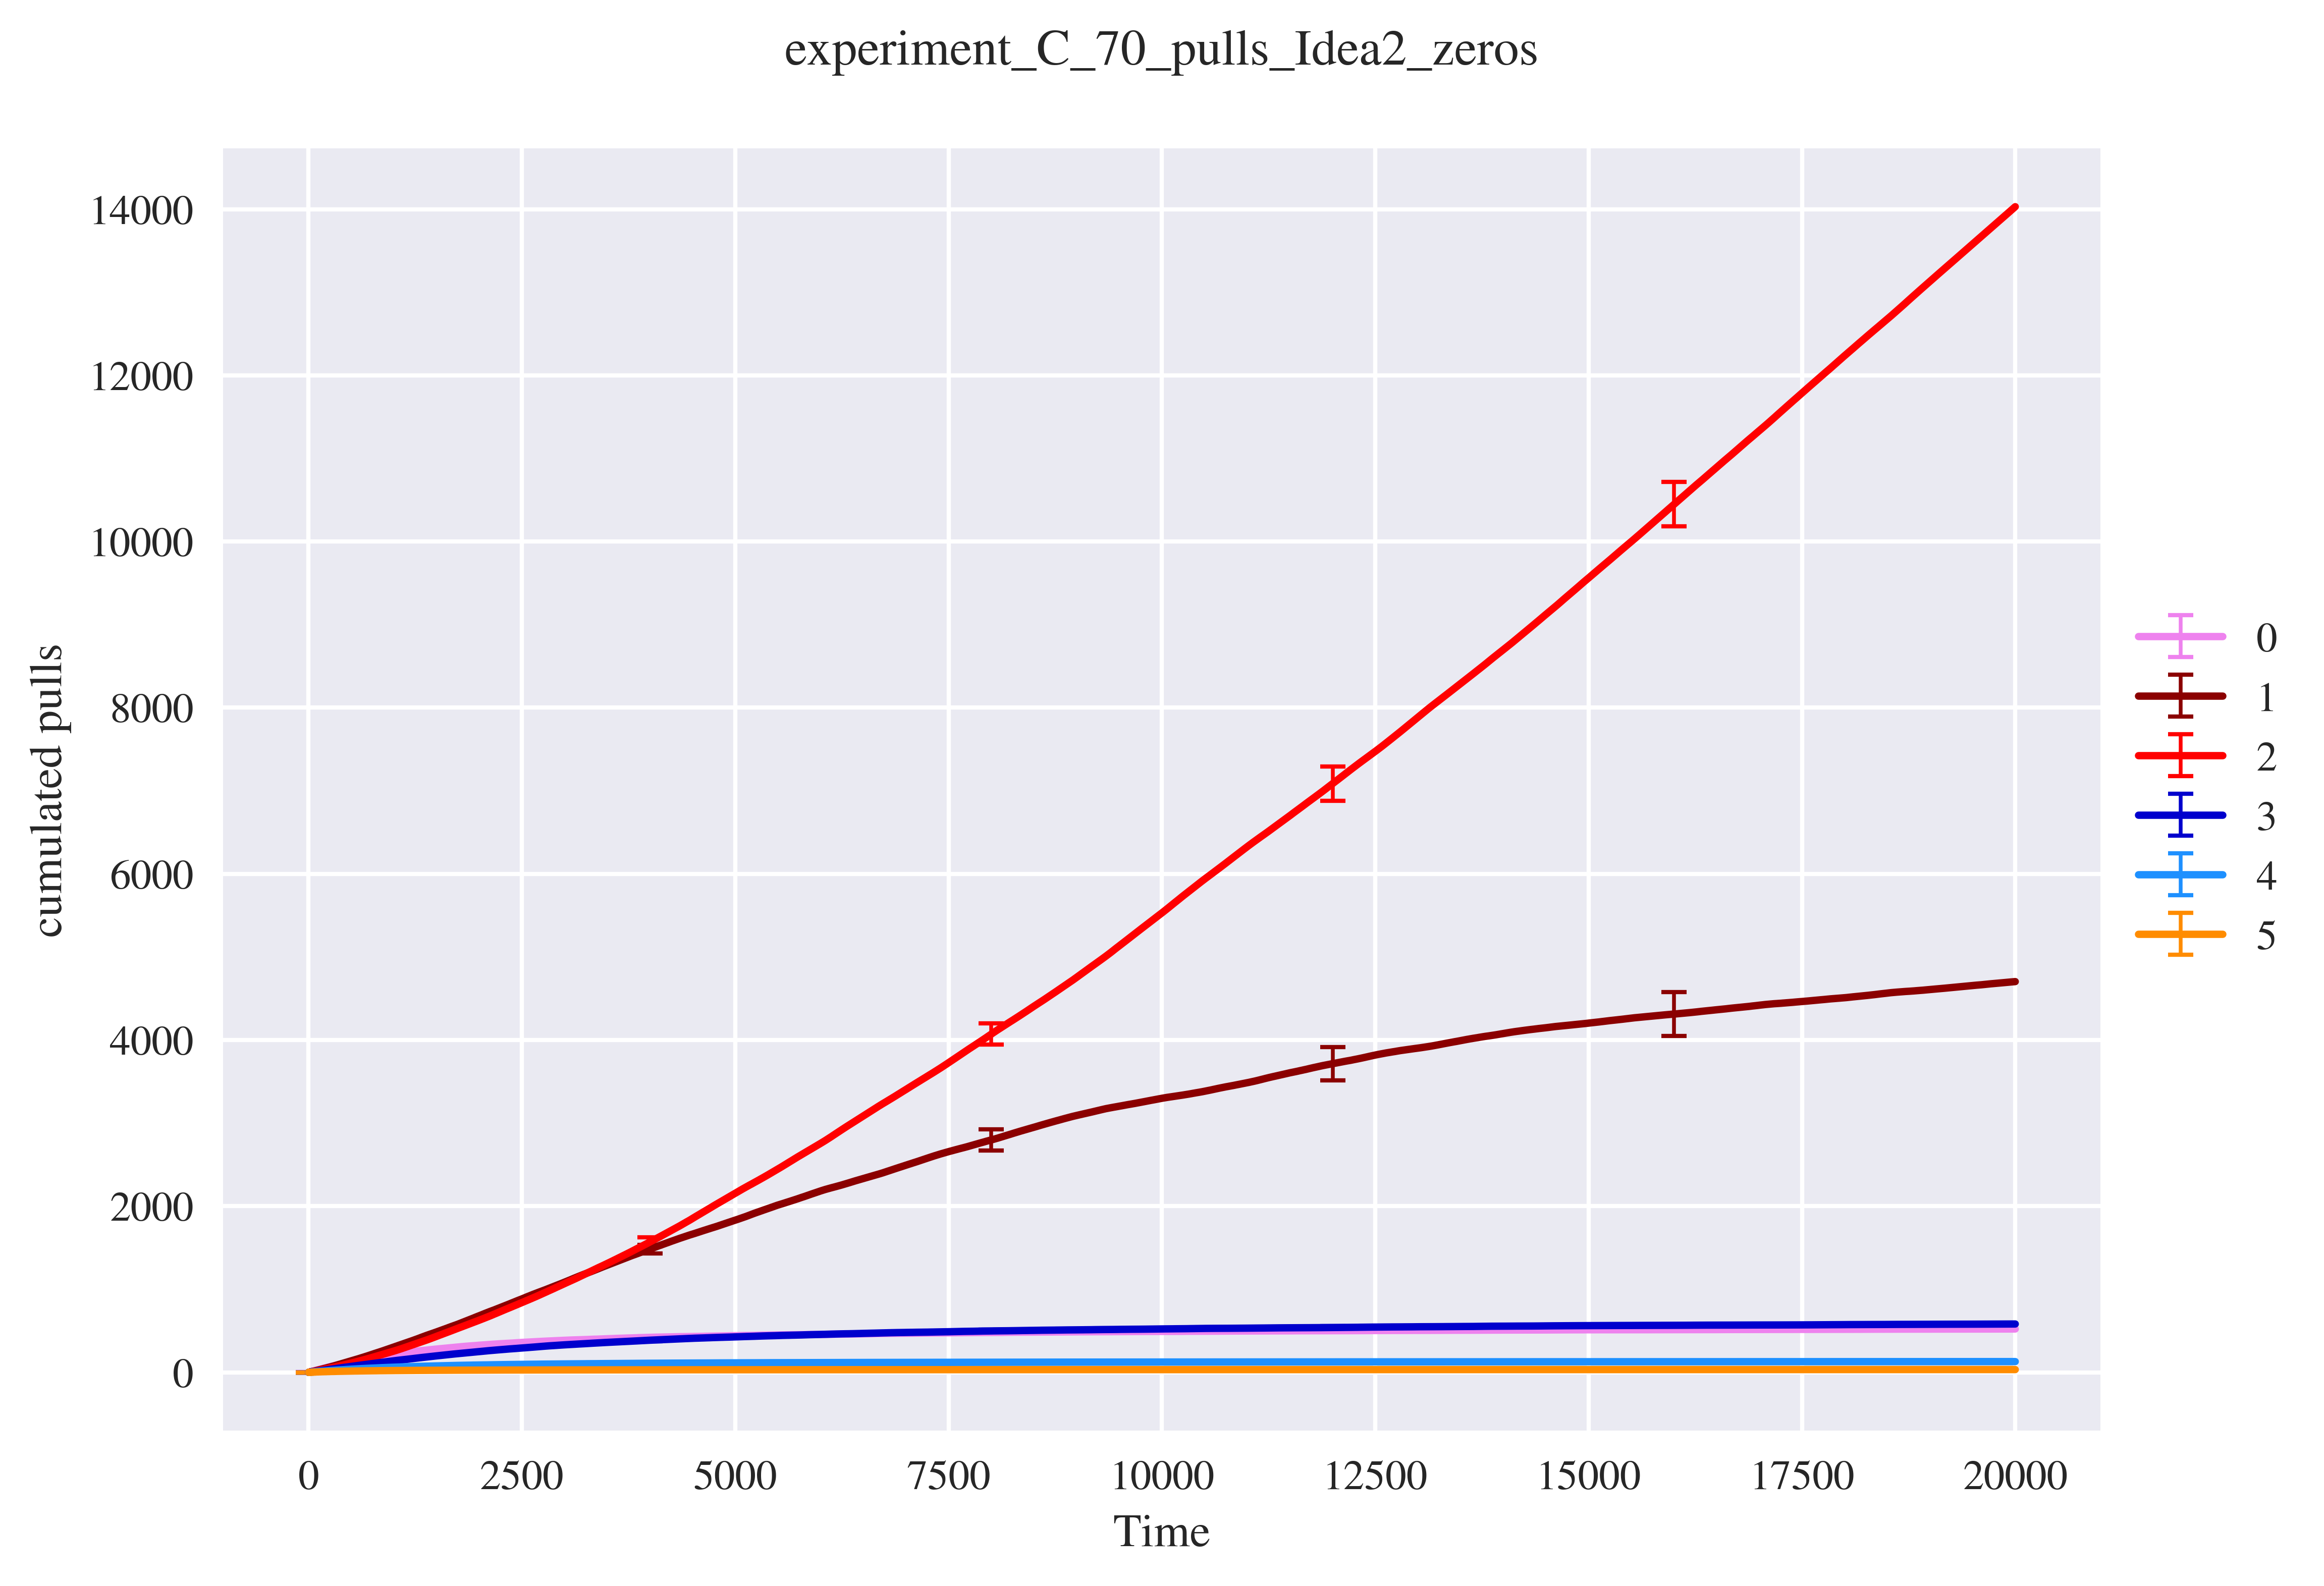
\includegraphics[width=6cm]{./images/PULLS/experiment_C_70Idea2_zeros cum_pulls.png}\quad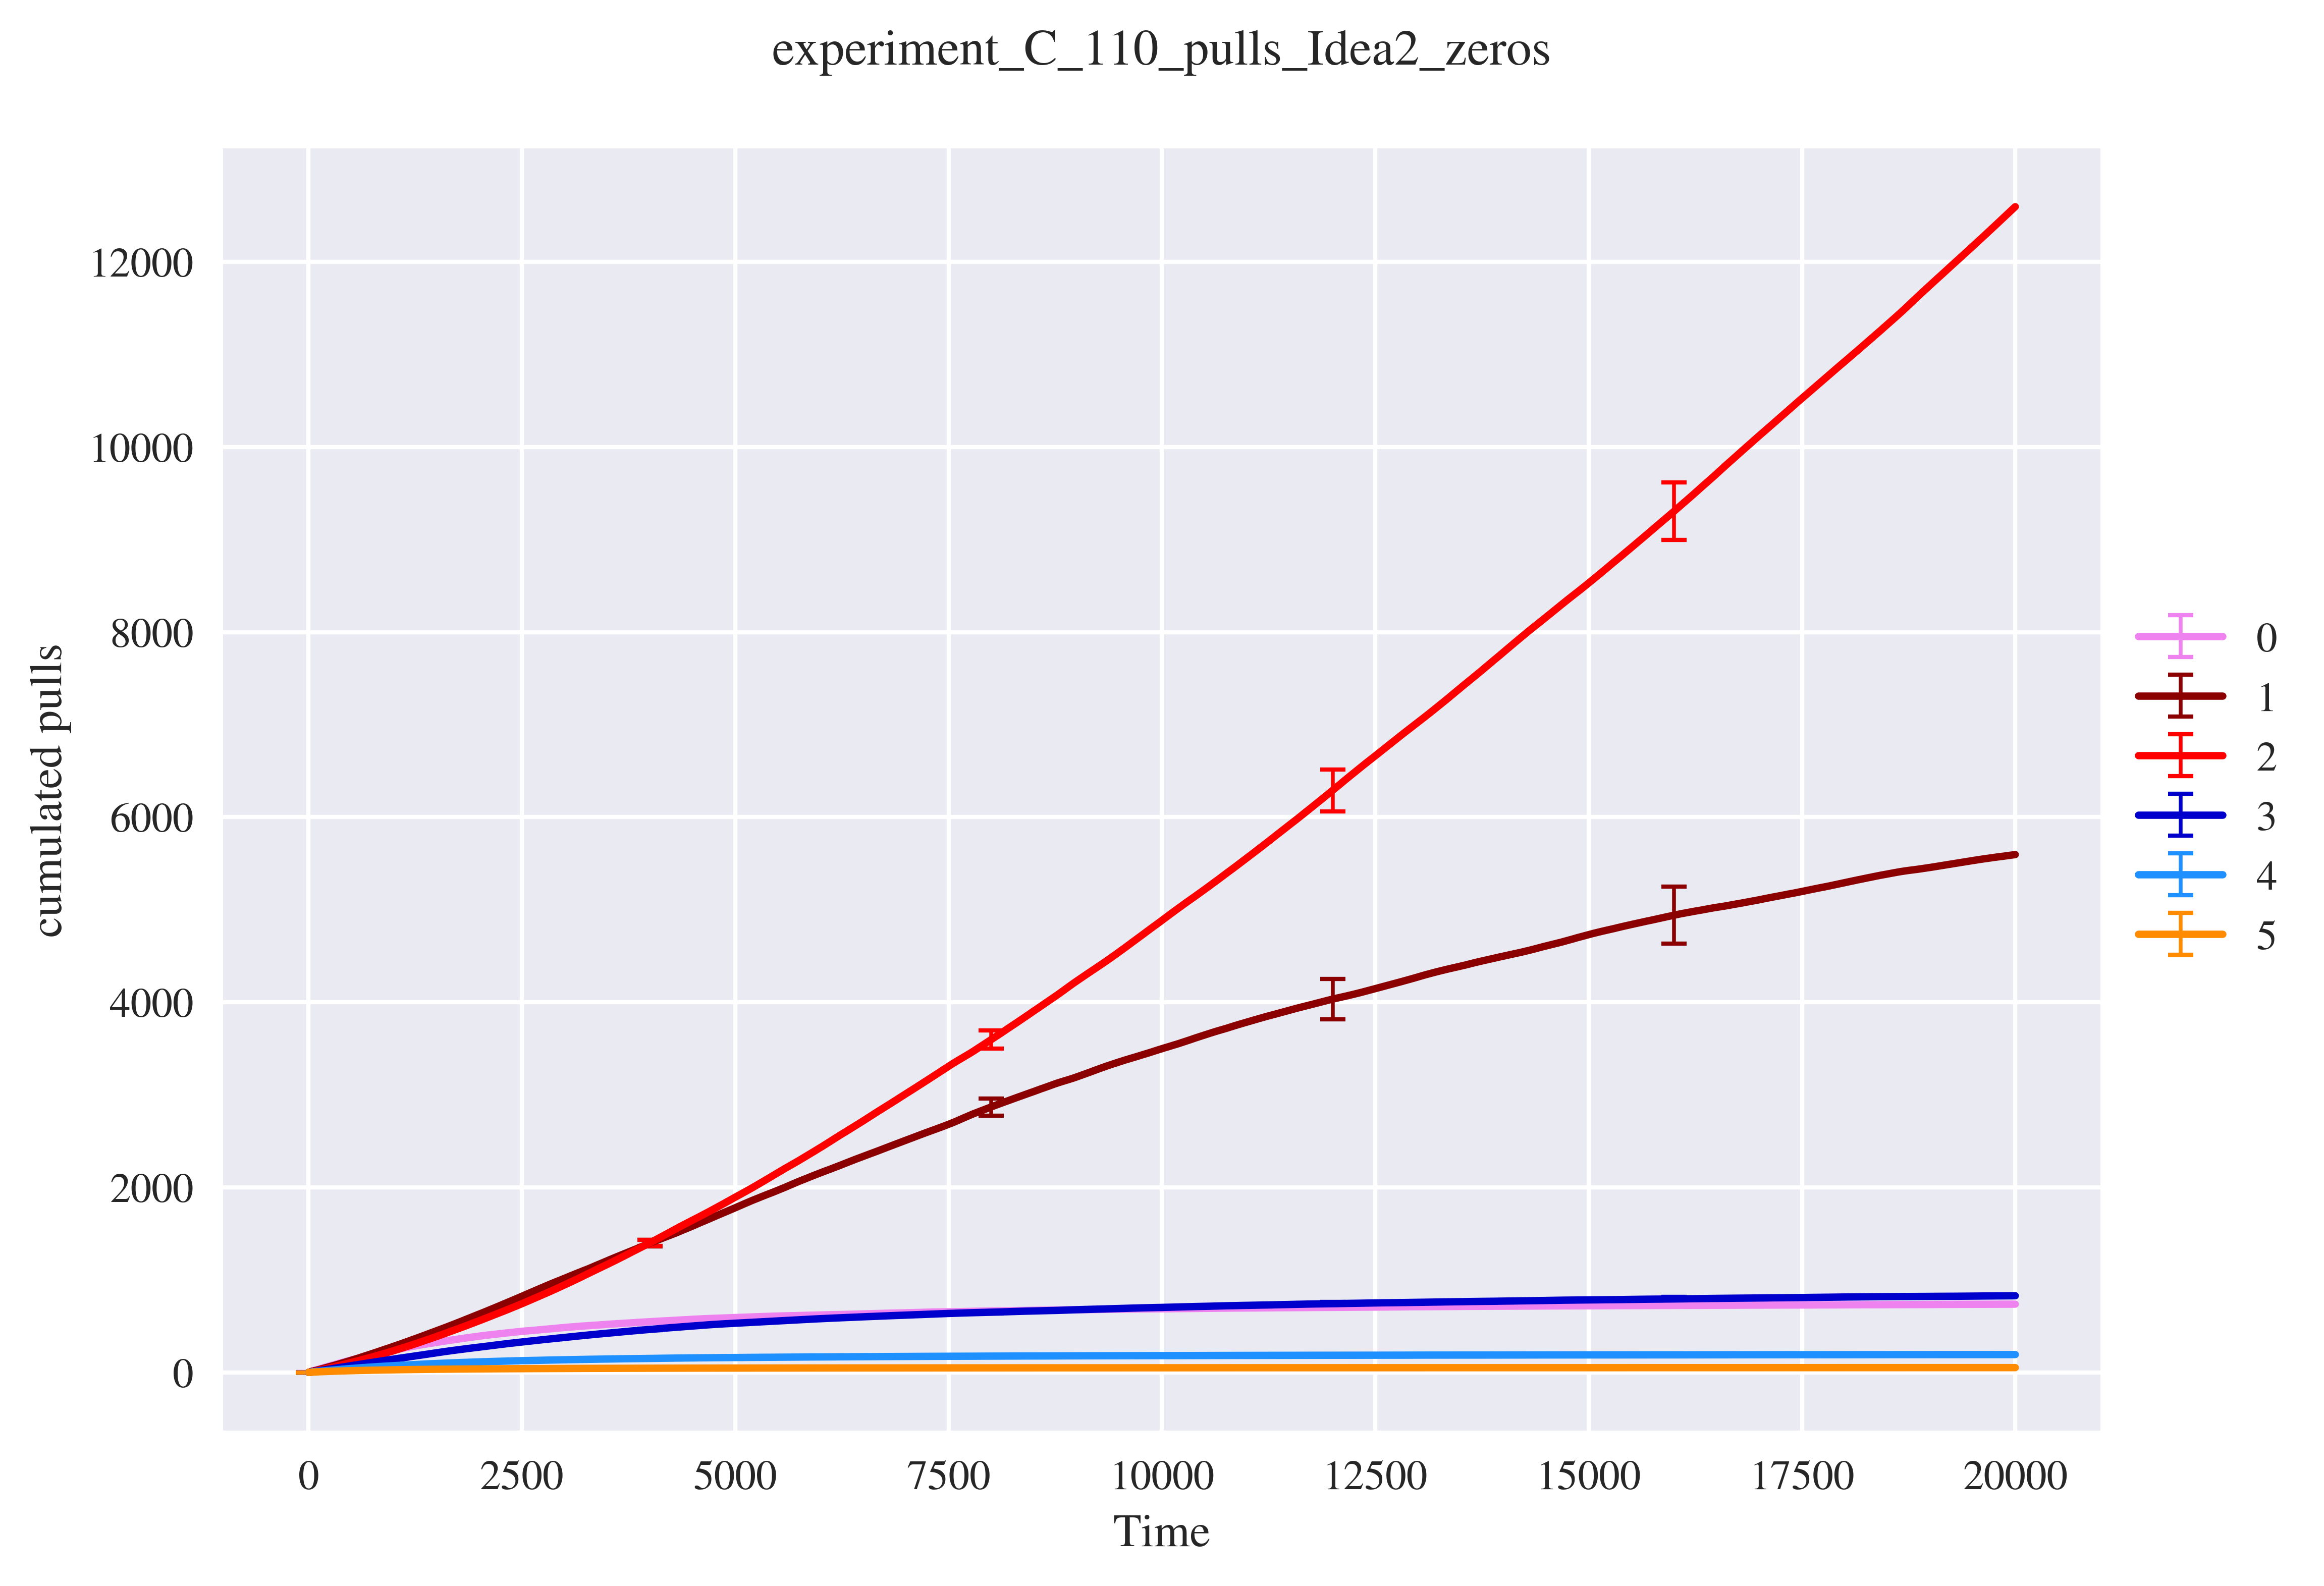
\includegraphics[width=6cm]{./images/PULLS/experiment_C_110Idea2_zeros cum_pulls.png}
	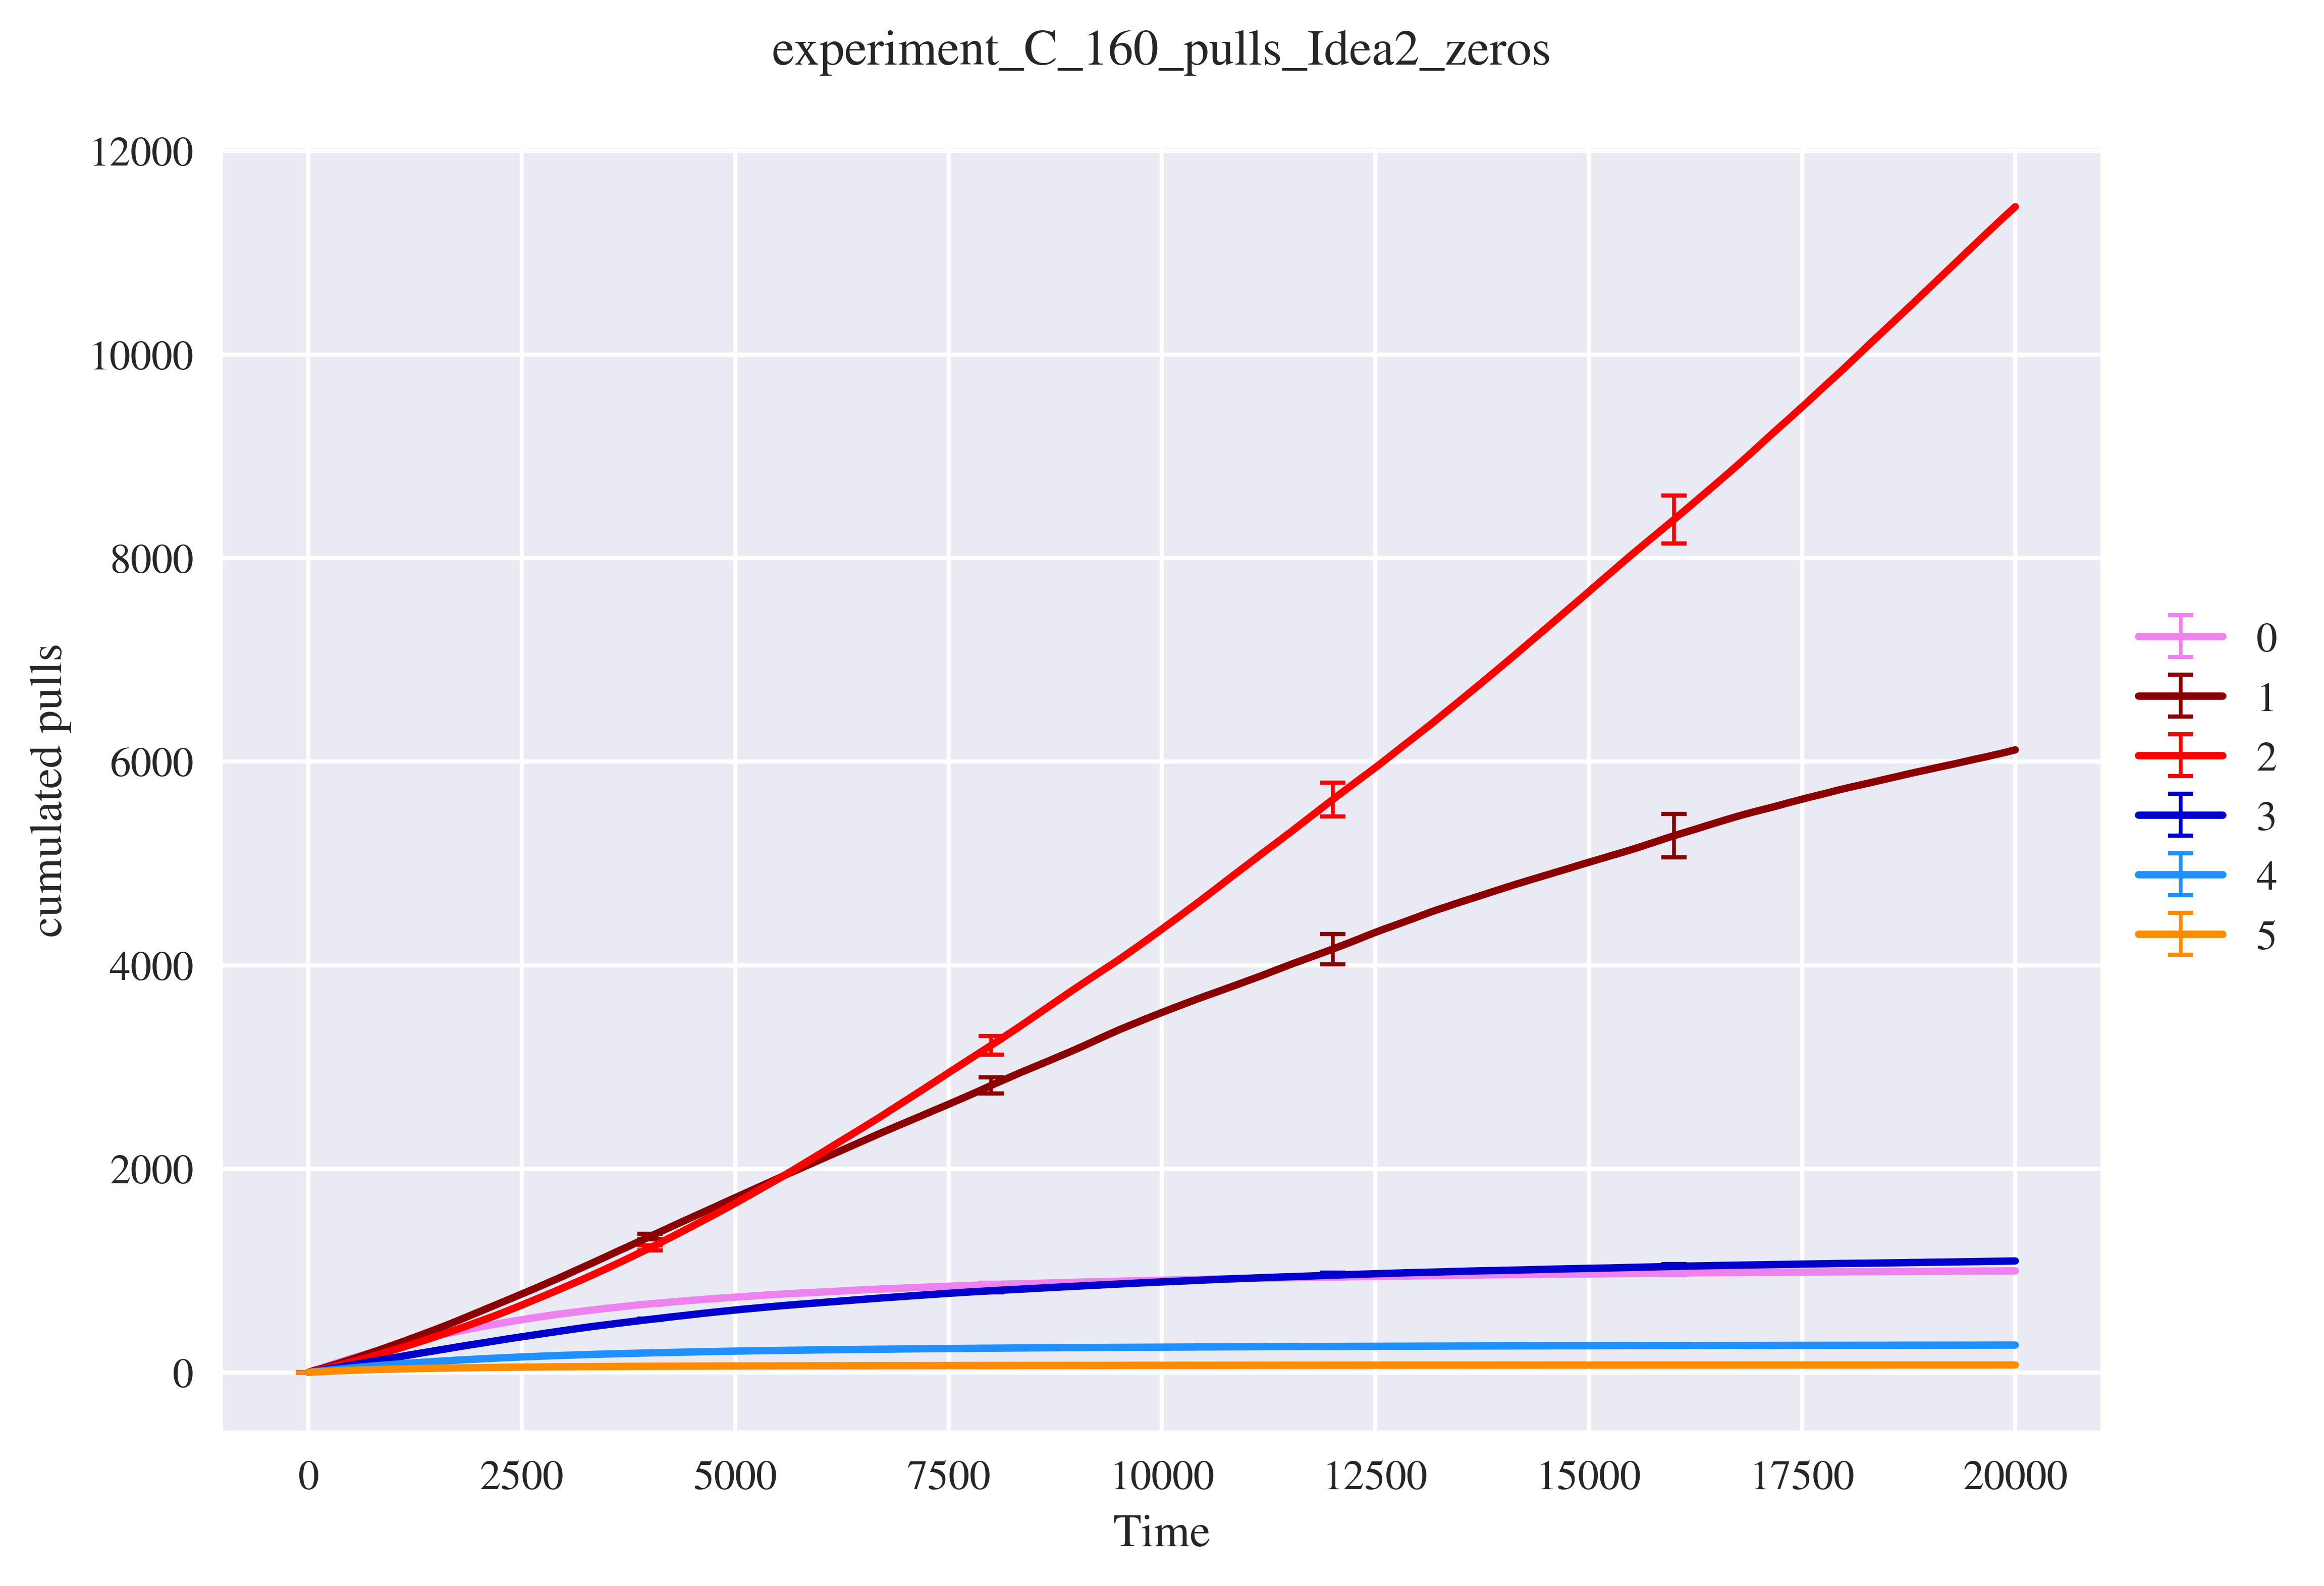
\includegraphics[width=6cm]{./images/PULLS/experiment_C_160Idea2_zeros cum_pulls.png}\quad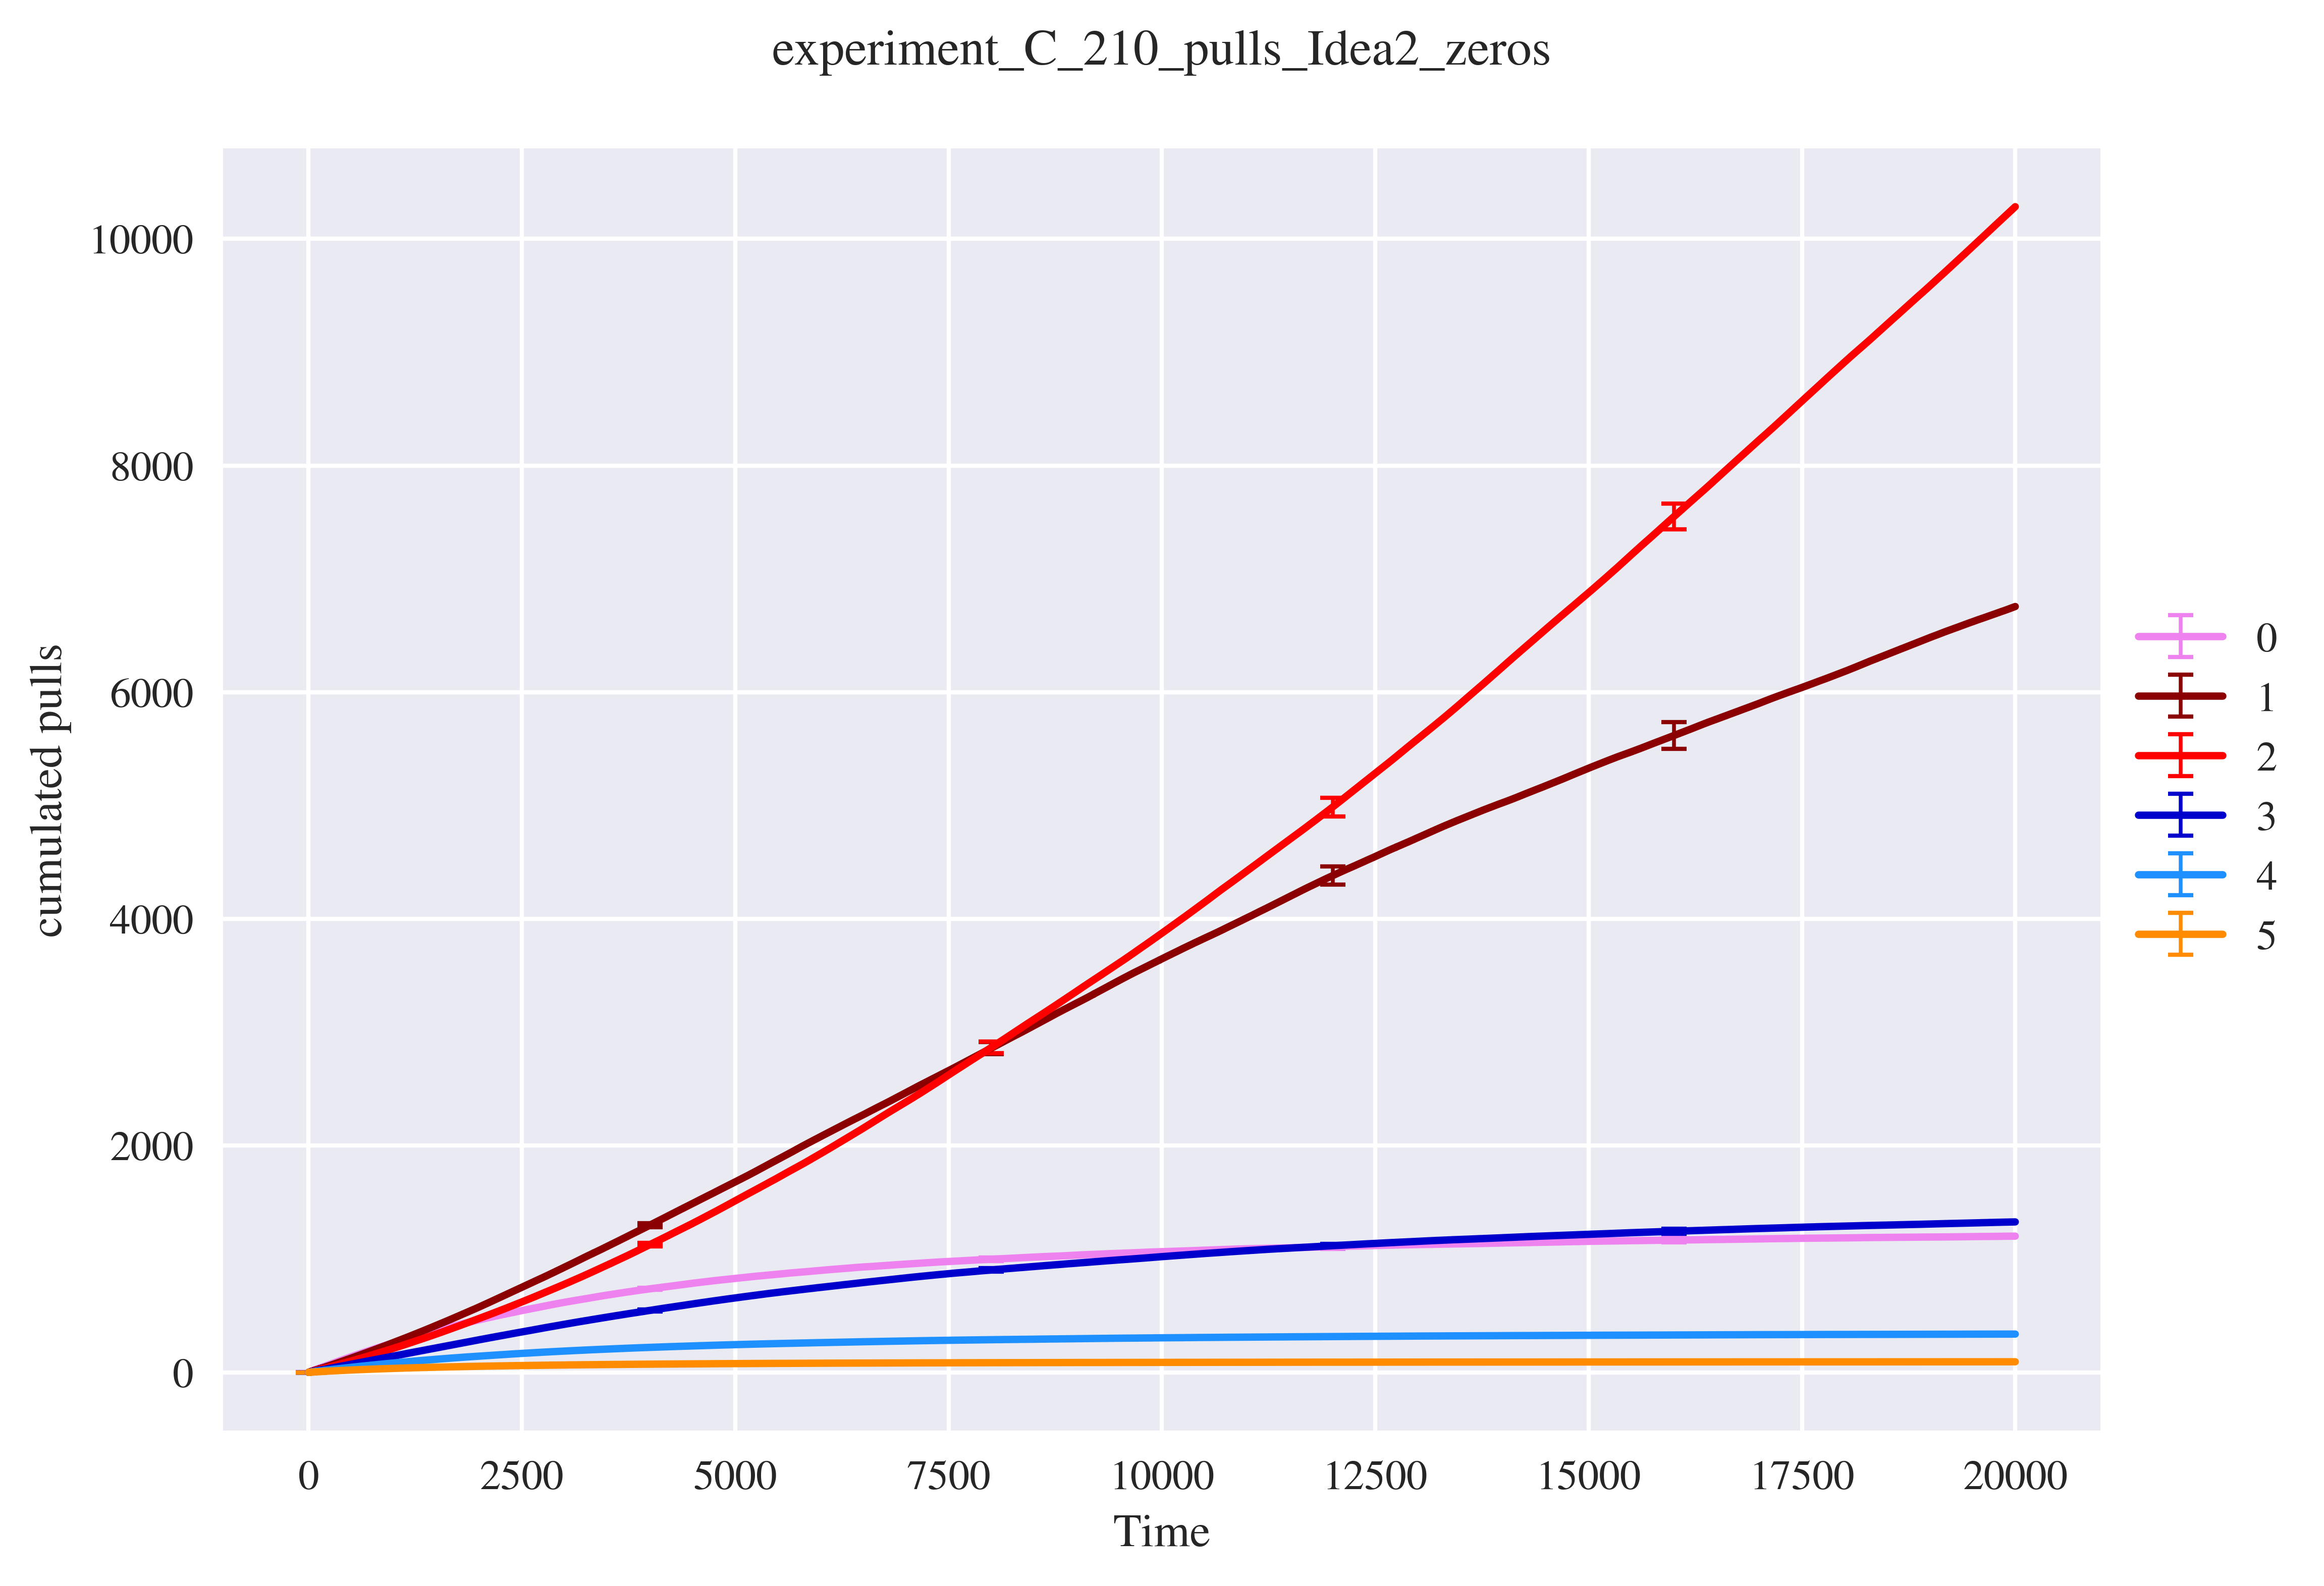
\includegraphics[width=6cm]{./images/PULLS/experiment_C_210Idea2_zeros cum_pulls.png}

	\caption{PULLS IDEA2 ZEROS C}
	
\end{figure}
